\documentclass[twoside,11pt]{article}

\usepackage{blindtext}

% Any additional packages needed should be included after jmlr2e.
% Note that jmlr2e.sty includes epsfig, amssymb, natbib and graphicx,
% and defines many common macros, such as 'proof' and 'example'.
%
% It also sets the bibliographystyle to plainnat; for more information on
% natbib citation styles, see the natbib documentation, a copy of which
% is archived at http://www.jmlr.org/format/natbib.pdf

% Available options for package jmlr2e are:
%
%   - abbrvbib : use abbrvnat for the bibliography style
%   - nohyperref : do not load the hyperref package
%   - preprint : remove JMLR specific information from the template,
%         useful for example for posting to preprint servers.
%
% Example of using the package with custom options:
%
% \usepackage[abbrvbib, preprint]{jmlr2e}

\usepackage[preprint]{jmlr2e}

\usepackage{amsfonts, amsmath, amssymb}
\usepackage{algorithm, algorithmicx, algpseudocode}
\usepackage{booktabs}

% Definitions of handy macros can go here

\newcommand{\dataset}{{\cal D}}
\newcommand{\fracpartial}[2]{\frac{\partial #1}{\partial  #2}}
\newcommand{\R}{\mathbb{R}}
\newcommand{\Sym}{\operatorname{Sym}}
\newcommand{\Skew}{\operatorname{Skew}}
\renewcommand{\O}{\mathcal{O}}
\renewcommand{\S}{\mathcal{S}}
\newcommand{\V}{\mathcal{V}}
\newcommand{\Sf}{\mathcal{S}_{1:d}}
\newcommand{\Uf}{U_{1:d}}
\newcommand{\qf}{q_{1:d}}
\newcommand{\SO}{\mathcal{SO}}
\newcommand{\diag}[1]{\operatorname{diag}\left(#1\right)}
\newcommand{\tr}[1]{\operatorname{tr}\left(#1\right)}
\newcommand{\norm}[1]{\left\lVert#1\right\rVert}
\newcommand{\lrp}[1]{\left(#1\right)}
\newcommand{\lrb}[1]{\left[#1\right]}
\newcommand{\lrs}[1]{\left\{#1\right\}}
\newcommand{\twodots}{\mathinner {\ldotp \ldotp}}
\newcommand{\St}{\operatorname{St}}
\newcommand{\Gr}{\operatorname{Gr}}
\newcommand{\Fl}{\operatorname{Fl}}
\newcommand{\T}{^\top}
\newcommand{\ambientstiefel}{\R^{n \times k}}
\newcommand{\argmin}[1]{\underset{#1}{\operatorname{argmin}} \, }
\newcommand{\argmax}[1]{\underset{#1}{\operatorname{argmax}} \, }
\newcommand{\N}[1]{\mathcal{N}\left(#1\right)}

% Heading arguments are {volume}{year}{pages}{date submitted}{date published}{paper id}{author-full-names}

\usepackage{lastpage}
\jmlrheading{23}{2024}{1-\pageref{LastPage}}{}{}{}{Tom Szwagier and Xavier Pennec}

% Short headings should be running head and authors last names

\ShortHeadings{Nested subspace learning with flags}{Szwagier and Pennec}
\firstpageno{1}

\begin{document}

\title{Nested subspace learning with flags}

\author{\name Tom Szwagier\email tom.szwagier@inria.fr \\
       \addr Université Côte d'Azur and Inria\\
       Sophia Antipolis, France
       \AND
       \name Xavier Pennec \email xavier.pennec@inria.fr \\
       \addr Université Côte d'Azur and Inria\\
       Sophia Antipolis, France}

\editor{}

\maketitle

\begin{abstract}%   <- trailing '%' for backward compatibility of .sty file
Many machine learning methods look for low-dimensional representations of the data. The underlying subspace can be estimated by {first} choosing a dimension $q$ and {then} optimizing a certain objective function over the space of $q$-dimensional subspaces---the Grassmannian. Trying different $q$ yields in general non-nested subspaces, which raises an important issue of consistency between the data representations. In this paper, we propose a simple trick to enforce nestedness in subspace learning methods. It consists in lifting Grassmannian optimization problems to flag manifolds---the space of nested subspaces of increasing dimension---via nested projectors. We apply the flag trick to several classical machine learning methods and show that it successfully addresses the nestedness issue.
\end{abstract}

\begin{keywords}
  subspace learning, Grassmann manifolds, flag manifolds, nested subspaces
\end{keywords}

\section{Introduction}


Sequential resource allocation is a fundamental problem in many domains, including healthcare, finance, and public policy \cite{considine2023optimizing,boehmer2024optimizing, yu2024fincon}. This task involves allocating limited resources over time while accounting for dynamic changes and competing demands. Deep reinforcement learning (RL) is an effective method to optimize decision-making for such challenges, offering efficient and scalable policies~\cite{yu2021reinforcement,talaat2022effective, xiong2023reinforcement,zhao2024towards}. However, deep RL policies generally provide action recommendations without human-readable reasoning and explanations. Such lack of interpretability poses a major challenge in critical domains where decisions must be transparent, justifiable, and in line with human decision-makers to ensure trust and compliance with ethical and regulatory standards.



For example, doctors may need to decide whether to prioritize intervention for Patient A or Patient B based on their current vital signs~\cite{boehmer2024optimizing}. An RL algorithm might suggest: \textit{ ``Intervene with Patient A "} with the implicit goal of maximizing the value function. However, the underlying reasoning may not be clear to the doctors, leaving them uncertain about the factors influencing the decision \cite{milani2024explainable}. For doctors, a more effective suggestion could be risk-based with specific information, e.g., \textit{``Patient A's vital signs are likely to deteriorate leading to higher potential risk compared to Patient B, so intervention with Patient A is prioritized"} \cite{gebrael2023enhancing, boatin2021wireless}.




\begin{figure*}[tbp]
    \centering
    \includegraphics[width=0.99\linewidth]{Figures/icml25_ProposedFramework.pdf}
    \caption{Overview of the \rbrl framework for joint sequential decision-making and explanation generation at time instance $t$. Starting with current state $\bs_t$,  a state-to-language descriptor generates \lang($\bs_t$), which is used to create the input prompt 
$\bp_t$. The LLM processes 
$\bp_t$
  to produce a thought 
$\pmb{\tau}_t$  and a set of candidate rules 
$\cR_t$ . An attention-based policy network selects a rule 
$\arule_t$ , which is used to derive an executable action $\aenv_t$ satisfying the budget constraint $B(\bs_t)$ for the environment 
  and a human-readable explanation $\pmb{\ell}_t^{expl}$, while also providing a rule reward $r_t^{\text{rule}}$ 
 . The environment transitions to the next state 
$\bs_{t+1}$ , returning an environment reward $r_t^{\text{env}}$ 
 . This process is repeated iteratively at subsequent time steps. 
}
    \label{fig:Proposed_framework}
\end{figure*}


Language agents \cite{sumers2024cognitive} leverage large language models (LLMs) for multi-step decision-making using reasoning techniques like chain of thought (CoT) \cite{wei2022chain} and ReAct \cite{yao2023react}. They enable natural language goal specification \cite{du2023guiding} and enhance human understanding \cite{hu2023language, srivastava2024policy}. However, LLMs struggle with complex sequential decision-making, such as resource allocation \cite{furuta2024exposing}, making RL a crucial tool for refining them into effective policy networks \cite{carta2023grounding, tantrue, wen2024reinforcing, zhai2024fine}. Yet, fine-tuning LLMs for policy learning is highly challenging due to the substantial computational costs and the complexity of token-level optimization \cite{rashid2024critical}, which remains an open challenge, particularly in sequential resource allocation.

Consequently, aiming to combine the strengths of both deep RL and language agents, we pose the following question:


\vspace{-0.1in}
\begin{tcolorbox}[colback=white!5!white,colframe=white!75!white]
\textit{%
Can we design a language agent framework that can simultaneously perform sequential resource allocation and provide human-readable explanations? }
\end{tcolorbox}
\vspace{-0.15in}






Motivated by existing work that employs predefined rules or concepts to explain RL policies \cite{Das2023State2Explanation} or guide RL exploration \cite{likmeta2020combining}, we explore the potential of using rules to prioritize individuals in resource allocation problems. In the context of language agents, rules are defined as ``structured statements" that capture prioritization among choices in a given state, aligning with the agent's goals \cite{srivastava2024policy}. 
Rules offer a flexible framework for encoding high-level decision criteria and priority logic, similar as the celebrated index policy for prioritizing arms in resource allocation problems \cite{whittle1988restless}, making them ideal for guiding resource allocation strategies while explaining the rationale behind decisions.%



Building on this, we propose a novel framework called Rule-Bottleneck Reinforcement Learning (\rbrl), which integrates the strengths of LLMs and RL to bridge the gap between decision-making and interoperability, by optimizing LLM-generated rules with RL. 
\rbrl provides a framework (as shown in Figure \ref{fig:Proposed_framework}) that simultaneously makes sequential resource allocation decisions and provides human-readable explanations. \rbrl leverages LLMs to generate candidate rules and employs RL to optimize policy selection, enabling the creation of effective decision policies while simultaneously providing human-understandable explanations. 

Our contributions are summarized as follows. \textit{First}, to avoid the computational cost and complexity of directly fine-tuning language agents, we leverage LLMs to generate a diverse set of rules, where each rule serves as a prioritization strategy for individuals in resource allocation. This approach enhances flexibility and interpretability in decision-making.
\textit{Second}, we extend the conventional state-action space by integrating the thoughts and rules generated by LLMs, creating a novel framework that enables reinforcement learning to operate on a richer, more interpretable decision structure.
\textit{Third}, we introduce an attention-based training framework that maps states to queries and rules to keys. The rule selection process is optimized by a policy network trained using the Soft Actor-Critic (SAC) algorithm \cite{haarnoja2018soft}, ensuring robust and efficient decision-making. In particular, the LLM also acts as a feedback mechanism, providing guidance during RL exploration to improve policy optimization and promote more effective learning. 
 



We evaluate our method in three environments from two real-world domains: \texttt{HeatAlerts}, where resources are allocated to mitigate extreme heat events; and \texttt{WearableDeviceAssignment}, for distributing monitoring devices to patients. 
Using cost-effective LLMs such as gpt-4o-mini \cite{openai2024gpt4omini} and Llama 3.1 8B \cite{meta2024llama3.1}, we first assess decision performance by comparing \rbrl with pure RL methods and language agent baselines. We then evaluate explanation quality through a human survey conducted under IRB approval. The results demonstrate \rbrl's effectiveness in both decision quality and interpretability.














\section{Reminders on flag manifolds}\label{sec:flags}

A flag is a sequence of nested linear subspaces of increasing dimension.
This section introduces flag manifolds and provides the minimal tools to perform optimization on those spaces. Much more details and properties can be obtained in dedicated papers~\citep{ye_optimization_2022}.

\subsection{Flags in the scientific literature}
By providing a natural parametrization for the eigenspaces of symmetric matrices, flags have long been geometrical objects of interest in the scientific community, with traditional applications in physics \citep{arnold_modes_1972} and linear algebra \citep{ammar_geometry_1986}.
Modern computational methods on flag manifolds arose later with the seminal work of \citet{edelman_geometry_1998} who provided some optimization algorithms on matrix manifolds such as Grassmannians and Stiefel manifolds.
Later, \citet{nishimori_riemannian_2006} provided an optimization algorithm on flag manifolds for independent subspace analysis \citep{cardoso_multidimensional_1998, hyvarinen_emergence_2000}.
Recently, flag manifolds played a central role in the investigation of a so-called \textit{curse of isotropy} in principal component analysis~\citep{szwagier_curse_2024}.

Flags as a sequence of nested subspaces were first introduced in the machine learning literature as robust prototypes to represent collections of subspaces of different dimensions~\citep{draper_flag_2014,mankovich_flag_2022}.
They were obtained via a sequential construction (where one dimension is added at a time), which can be problematic for greediness reasons~\citep{huber_projection_1985,lerman_overview_2018}.
\citet{pennec_barycentric_2018} was the first to show that PCA can be reformulated as an optimization problem on flag manifolds by summing the unexplained variance at different dimensions. This principle was recently applied to several variants of PCA under the name of \textit{flagification} in~\citet{mankovich_fun_2024}, showing an important robustness to outliers.
Finally, some works compute distance-related quantities on flag-valued datasets, with notable applications in computer vision and hyperspectral imaging~\citep{ma_flag_2021, nguyen_closed-form_2022, mankovich_chordal_2023, szwagier_rethinking_2023}.


\subsection{Definition and representation of flag manifolds}
Let $p \geq 2$ %be an ambient dimension 
and $q_{1:d} := (q_1, q_2 ,\cdots, q_d)$ be a sequence of increasing integers such that $~{0 < q_1 < q_2 < \cdots < q_d < p}$.
A \textit{flag} of \textit{signature} $(p, q_{1:d})$ is a sequence of nested {linear} subspaces $\{0\} \subset \S_1 \subset \S_2 \subset \dots \subset \S_d \subset \R^p$ of respective dimension $q_1, q_2, \dots, q_d$, noted here $\S_{1:d} := (\S_1, \dots, \S_d)$.\footnote{Flags can equivalently be defined as sequences of \textit{mutually orthogonal} subspaces $\V_1 \perp \V_2 \dots \perp \V_d$, of respective dimension $q_1, q_2-q_1, \dots, q_d - q_{d-1}$, by taking $\V_k$ to be the orthonormal complement of $\S_{k-1}$ onto $\S_k$. This definition is more convenient for computations, but it won't be the one used in this paper.}
A flag $\S_{1:d}$ can be canonically represented as a sequence of symmetric matrices that are the \textit{orthogonal projection matrices} onto the nested subspaces, i.e. $\S_{1:d} \cong (\Pi_{\S_1}, \dots, \Pi_{\S_d})\in\Sym_p^d$. We call it the \textit{projection representation} of flags.

The set of flags of signature $(p, q_{1:d})$ is a smooth manifold~\citep{ye_optimization_2022}, denoted here $\Fl(p, q_{1:d})$. 
Flag manifolds generalize {Grassmannians}---since $~{\Fl(p, (q,)) = \Gr(p, q)}$---and therefore share many practical properties that are useful for optimization~\citep{edelman_geometry_1998}. In the following, we will frequently use the following notations: $q_0 := 0$, $q := q_d$ and $q_{d+1} := p$.


For computational and numerical reasons, flags are often represented as orthonormal $q$-frames. Those correspond to points on the Stiefel manifold $\St(p, q) = \{U\in\R^{p\times q}\colon U\T U = I_q\}$).
Let us define sequentially, for $k\in[1, d]$, $U_k\in\St(p, q_k - q_{k-1})$ such that $[U_1|\dots|U_k]$ is an orthonormal basis of $\S_k$ (this is possible thanks to the nestedness of the subspaces).
Then, $U_{1:d} := [U_1|\dots|U_d]\in\St(p, q)$ is a representative of the flag $\S_{1:d}$. We call it the \textit{Stiefel representation} of flags. Such a representation is not unique---contrary to the projection representation defined previously---due to the \textit{rotational-invariance} of orthonormal bases of subspaces. More precisely, if $U_{1:d}$ is a Stiefel representative of the flag $\S_{1:d}$, then for any set of orthogonal matrices $R_k\in\O(q_k - q_{k-1})$, the matrix $U'_{1:d} := [U_1 R_1|\dots|U_d R_d]$ spans the same flag of subspaces $\S_{1:d}$.
This provides flag manifolds with a quotient manifold structure~\citep{edelman_geometry_1998, absil_optimization_2009, ye_optimization_2022}: 
\begin{equation}\label{eq:Fl_quotient}
	\Fl(p, q_{1:d}) \cong \St(p, q) \big/ \lrp{\O(q_1) \times \O(q_2 - q_1) \times \dots \times \O(q_d - q_{d-1})}.
\end{equation}

\begin{remark}[Orthogonal representation]
For computations, one might have to perform the orthogonal completion of some Stiefel representatives.
Let $\Uf := [U_1|\dots|U_d] \in \St(p, q)$, then one denotes $U_{d+1} \in \St(p, p-q_d)$ to be any orthonormal basis such that $U_{1:d+1} := [U_1|\dots|U_d|U_{d+1}] \in \O(p)$. Such an orthogonal matrix $U_{1:d+1}$ will be called an \emph{orthogonal representative} of the flag $\Sf$. In the following, we may abusively switch from one representation to the other since they represent the same flag.
\end{remark}

\subsection{Optimization on flag manifolds}
There is a rich literature on optimization on smooth manifolds~\citep{edelman_geometry_1998,absil_optimization_2009,boumal_introduction_2023}, and the particular case of flag manifolds has been notably addressed in~\citet{ye_optimization_2022,zhu_practical_2024}. Since flag manifolds can be represented as quotient spaces of Stiefel manifolds, which themselves are embedded in a Euclidean matrix space, one can develop some optimization algorithms without much difficulty.
In this paper, we will use a \textit{steepest descent} algorithm, which is drawn from several works~\citep{chikuse_statistics_2003,nishimori_riemannian_2006,ye_optimization_2022,zhu_practical_2024}. 
Let $f\colon \Fl(p, \qf) \to \R$ be a smooth function on a flag manifold, expressed in the Stiefel representation (e.g. $f(\Uf) = \sum_{k=1}^d \norm{{U_k} {U_k}\T x} $ for some $x\in\R^p$). Given $\Uf \in \St(p, q)$, let $\operatorname{Grad} f (\Uf) = ({\partial f}/{\partial U_{ij}})_{i, j = 1}^{p, q}$ denote the (Euclidean) gradient of $f$. To ``stay'' on the manifold, one first computes the \textit{Riemannian gradient} of $f$ at $\Uf$, noted $\nabla f (\Uf)$. It can be thought of as a projection of the Euclidean gradient onto the tangent space and computed explicitly~\citep{nishimori_riemannian_2006,ye_optimization_2022}.
Then, one moves in the opposite direction of $\nabla f (\Uf)$ with a so-called \textit{retraction}, which is chosen to be the polar retraction of~\citet[Eq.~(49)]{zhu_practical_2024}, combined with a line-search.
We iterate until convergence.
The final steepest descent algorithm is described in Algorithm~\ref{alg:GD}.
\begin{algorithm}
\caption{Steepest descent on flag manifolds}\label{alg:GD}
\begin{algorithmic}
\Require $f\colon \Fl(p, \qf) \to \R$ a function, $\Uf \in \Fl(p, \qf)$ a flag (Stiefel representation)
\For{$t$ = 1, 2, \dots}
    \State $[G_1|\dots|G_d] \gets \operatorname{Grad} f (\Uf)$ \Comment{Euclidean gradient}
	\State $\nabla \gets \bigl[G_k - \bigl(U_k {U_k}\T G_k + \sum_{l \neq k} U_l {G_l}\T U_k\bigr)\bigr]_{k=1\dots d}$
	\Comment{Riemannian gradient}
	\State $\Uf \gets \operatorname{polar}(U_{1:d+1} - \alpha \nabla)$ \Comment{polar retraction + line search}
\EndFor
\Ensure $U_{1:d}^* \in \Fl(p, \qf)$ an optimal flag
\end{algorithmic}
\end{algorithm}
\begin{remark}[Initialization]
We can initialize Algorithm~\ref{alg:GD} randomly via~\citet[Theorem~1.5.5]{chikuse_statistics_2003}, or choose a specific flag depending on the application, as we will see in \autoref{sec:examples}.
\end{remark}
\begin{remark}[Optimization variants]\label{rk:optim}
Many extensions of Algorithm~\ref{alg:GD} can be considered: conjugate gradient~\citep{ye_optimization_2022}, Riemannian trust region~\citep{absil_optimization_2009} etc. We can also replace the polar retraction with a geodesic step~\citep{ye_optimization_2022} or other retractions~\citep{zhu_practical_2024}.
\end{remark}
 \section{The flag trick in theory}\label{sec:flag_trick}
In this section, we motivate and introduce the flag trick to make subspace learning methods nested.
The key result is \autoref{thm:flag_trick}, which states that the classical PCA at a fixed dimension can be converted into a nested multilevel method using nested projectors.

In the remaining of the paper, we assume that the data has been already \textit{centered} around a point of interest (e.g. its mean or geometric median), so that we are only interested in fitting \textit{linear} subspaces and not \textit{affine} ones. 
One could directly include the center in the optimization variables---in which case the geometry would be the one of affine Grassmannians~\citep{lim_numerical_2019} or affine flags~\citep{pennec_barycentric_2018}---but we don't do it in this work for conciseness.


\subsection{From subspaces to flags of subspaces: the seminal example of PCA}
PCA is known as the eigendecomposition of the sample covariance matrix. Originally, it can be formulated as the search for a low dimensional subspace that minimizes the unexplained variance (or maximizes the explained variance).
Let $X:=[x_1|\dots|x_n] \in \R^{p\times n}$ be a data matrix with $n$ samples, let $\S \in \Gr(p, q)$ be a $q$-dimensional subspace, and let $\Pi_{\S} \in \R^{p\times p}$ be the orthogonal projection matrix onto $\S$.
Then PCA consists in the following optimization problem on Grassmannians:
\begin{equation}\label{eq:PCA_subspace}
\S_q^* = \argmin{\S \in \Gr(p, q)} \norm{X - \Pi_{\S} X}_F^2,
\end{equation}
where $\norm{M}_F^2 := \tr{M\T M}$ denotes the \textit{Frobenius norm}.
The solution to the optimization problem is the $q$-dimensional subspace spanned by the leading eigenvectors of the sample covariance matrix $S := \frac 1 n X X\T$, that we note $\S_q^* = \operatorname{Span}(v_1, \dots, v_q)$. 
It is unique when the sample eigenvalues $q$ and $q+1$ are distinct, which is almost sure when $q \leq \operatorname{rank}(S)$. We will assume to be in such a setting in the following for simplicity but it can be easily handled otherwise by ``grouping'' the repeated eigenvalues (cf.~\citet[Theorem~B.1]{szwagier_curse_2024}).
In such a case, the principal subspaces are \textit{nested} for increasing $q$, i.e., if $\S_q^*$ is the $q$-dimensional principal subspace, then for any $r > q$, one has $\S_q^* = \operatorname{Span}(v_1, \dots, v_q) \subset \operatorname{Span}(v_1, \dots, v_r) = \S_r^*$.

Another way of performing PCA is in a sequential manner (cf. footnote~\ref{footnote:sequential}). We first estimate the 1D subspace $\mathcal{V}_1^*$ that minimizes the unexplained variance, then estimate the 1D subspace $\mathcal{V}_2^*$ that minimizes the unexplained variance while being orthogonal to the previous one, and so on and so forth. This gives the following \textit{constrained} optimization problem on 1D Grassmannians:
\begin{equation}\label{eq:PCA_sequential}
\mathcal{V}_q^* = \argmin{\substack{\mathcal{V} \in \Gr(p, 1)\\ \mathcal{V} \perp \mathcal{V}_{q-1} \perp \dots \perp \mathcal{V}_1}} \norm{X - \Pi_{\mathcal{V}} X}_F^2.
\end{equation}
This construction naturally yields a sequence of nested subspaces of increasing dimension---i.e. a flag of subspaces---best and best approximating the dataset:
\begin{equation}
	\{0\} \subset \S_1^* \subset \S_2^* \subset \dots \subset \S_{p-1}^* \subset \R^p, \text{with } \S_k^* = \bigoplus_{l=1}^k \mathcal{V}_l^*.
\end{equation}
Those subspaces happen to be exactly the same as the ones obtained by solving the subspace learning optimization problem~\eqref{eq:PCA_subspace}, although the way they are obtained (in a greedy manner) is different. This is generally not the case for other dimension reduction problems (for instance in robust subspace recovery, as it is raised in the final open questions of~\citet{lerman_overview_2018}).

Hence, the optimal solution to the \textit{subspace} learning formulation of PCA~\eqref{eq:PCA_subspace} is equivalent to the \textit{sequential} formulation of PCA~\eqref{eq:PCA_sequential}, and both yield a flag of subspaces best and best approximating the data. One can wonder if this result could be directly obtained by formulating an optimization problem on flag manifolds. The answer is \textit{yes}, as first proven in~\citet[Theorem~9]{pennec_barycentric_2018} with an \textit{accumulated unexplained variance} (AUV) technique, but there is not a unique way to do it. Motivated by the recent principal subspace analysis~\citep{szwagier_curse_2024}, we propose in the following theorem a generic trick to formulate PCA as an optimization on flag manifolds.
\begin{theorem}[Nested PCA with flag manifolds]\label{thm:flag_trick}
	Let $X := [x_1|\dots|x_n]\in\R^{p\times n}$ be a centered $p$-dimensional ($p \geq 2$) dataset with $n$ samples. Let $q_{1:d} := (q_1, q_2 ,\cdots, q_d)$ be a sequence of increasing dimensions such that $0 < q_1 < q_2 < \cdots < q_d < p$.
	Let $S := \frac 1 n X X\T$ be the sample covariance matrix. Assume that it eigendecomposes as $S := \sum_{j=1}^p \ell_j v_j {v_j}\T$ where $\ell_1 \geq \dots \geq \ell_p$ are the eigenvalues and $v_1 \perp \dots \perp v_p$ are the associated eigenvectors.
	Then PCA can be reformulated as the following optimization problem on flag manifolds:
	\begin{equation}
		{\S_{1:d}^*} = \argmin{\S_{1:d} \in \Fl(p, q_{1:d})} \norm{X - \frac 1 d \sum_{k=1}^d \Pi_{\S_k} X}_F^2.
	\end{equation}
	More precisely, one has ${\S_{1:d}^*} = \lrp{\operatorname{Span}(v_1, \dots, v_{q_1}), \operatorname{Span}(v_1, \dots, v_{q_2}), \dots, \operatorname{Span}(v_1, \dots, v_{q_d})}$.
	The solution is unique if and only if $\ell_{q_k} \neq \ell_{q_{k+1}}, \forall k\in[1, d]$.
\end{theorem}
\begin{proof} 
One has:
\begin{align}
	\norm{X - \frac 1 d \sum_{k=1}^d \Pi_{\S_k} X}_F^2
	&= \tr{X\T \lrp{I_p - \frac1d\sum_{k=1}^d \Pi_{\S_k}}^2 X},\\
	&= \frac1{d^2} \tr{X\T \lrp{\sum_{k=1}^d \lrp{I_p - \Pi_{\S_k}}}^2 X},\\
	&= \frac n {d^2} \tr{W^2 S},
\end{align}
with $W = \sum_{k=1}^d (I_p - \Pi_{\S_k})$ and $S = \frac 1 n X X\T$.
	Let $U_{1:d+1} := [U_1|\dots|U_d|U_{d+1}]\in\O(p)$ be an orthogonal representative (cf. \autoref{sec:flags}) of the optimization variable $\S_{1:d} \in \Fl(p, q_{1:d})$. Then one has $~{\Pi_{\S_k} = U_{1:d+1} \diag{I_{q_k}, 0_{p - q_k}} {U_{1:d+1}}\T}$. Therefore, one has $W = U_{1:d+1} \Lambda {U_{1:d+1}}\T$, with $~{\Lambda = \diag{0 \, I_{q_1}, 1 \, I_{q_2 - q_1}, \dots, d \, I_{q_{d+1} - q_d}}}$.
	Hence, one has 
	\begin{equation}
		\argmin{\S_{1:d} \in \Fl(p, q_{1:d})} \norm{X - \frac 1 d \sum_{k=1}^d \Pi_{\S_k} X}_F^2 \Longleftrightarrow \argmin{U \in \O(p)} \frac n {d^2} \tr{U \Lambda^2 U\T S}.
	\end{equation}
	The latter problem is exactly the same as in~\citet[Equation~(19)]{szwagier_curse_2024}, which solves maximum likelihood estimation for principal subspace analysis.
	Hence, one can conclude the proof on existence and uniqueness using~\citet[Theorem~B.1]{szwagier_curse_2024}.
\end{proof}
The key element of the proof of \autoref{thm:flag_trick} is that averaging the nested projectors yields a \textit{hierarchical reweighting} of the (mutually-orthogonal) principal subspaces. More precisely, the $k$-th principal subspace has weight $(k-1)^2$, and this reweighting enables to get a hierarchy of eigenspaces~\citep{cunningham_linear_2015,pennec_barycentric_2018,oftadeh_eliminating_2020}.
In the following, we note $~{\Pi_{\S_{1:d}} := \frac 1 d \sum_{k=1}^d \Pi_{\S_k}}$ and call this symmetric matrix the \textit{average multilevel projector}, which will be central in the extension of subspace methods into multilevel subspace methods.



\subsection{The flag trick}
As we will see in the following (\autoref{sec:examples}), many important machine learning problems can be formulated as the optimization of a certain function $f$ on Grassmannians.
\autoref{thm:flag_trick} shows that replacing the subspace projection matrix $\Pi_{\S}$ appearing in the objective function by the average multilevel projector $\Pi_{\Sf}$ yields a sequence of subspaces that meet the original objective of principal component analysis, while being nested.
This leads us to introduce the \textit{flag trick} for general subspace learning problems.
\begin{definition}[Flag trick]\label{def:flag_trick}
Let $p \geq 2$, $0 < q < p$ and $q_{1:d} := (q_1, q_2 ,\cdots, q_d)$ be a sequence of increasing dimensions such that $0 < q_1 < q_2 < \cdots < q_d < p$.
The flag trick consists in replacing a subspace learning problem of the form:
\begin{equation}\label{eq:subspace_problem}
    \argmin{\S \in \Gr(p, q)} f(\Pi_\S)
\end{equation}
with the following optimization problem:
\begin{equation}\label{eq:flag_problem}
    \argmin{\S_{1:d} \in \Fl(p, q_{1:d})} f\lrp{\frac 1 d \sum_{k=1}^d \Pi_{\S_k}}.
\end{equation}
\end{definition}
Except for the very particular case of PCA (\autoref{thm:flag_trick}) where $f_X(\Pi) = \norm{X - \Pi X}_F^2$, we cannot expect to have an analytic solution to the flag problem~\eqref{eq:flag_problem}; indeed, in general, subspace problems do not even have a closed-form solution as we shall see in \autoref{sec:examples}. This justifies the introduction of optimization algorithms on flag manifolds like Algorithm~\ref{alg:GD}. 

\begin{remark}[Flag trick vs. AUV]
The original idea of accumulated unexplained variance~\citep{pennec_barycentric_2018} (and its subsequent application to several variants of PCA under the name of ``flagification''~\citep{mankovich_fun_2024}) consists in summing the subspace criteria at different dimensions, while the flag trick directly averages the orthogonal projection matrices that appear inside the objective function.
While both ideas are equally worth experimenting with, we believe that the flag trick has a much wider reach. Indeed, from a technical viewpoint, the flag trick appears at the covariance level and directly yields a hierarchical reweighting of the principal subspaces. This reweighting is only indirect with the AUV---due to the linearity of the trace operator---and is not expected to happen for other methods than PCA. Notably, as we shall see in \autoref{sec:examples}, the flag trick enables to easily develop extensions of well-known methods involving PCA, like IRLS~\citep{lerman_fast_2018} or Newton-Lanczos methods for trace ratio optimization~\citep{ngo_trace_2012}, and is closer in spirit to the statistical formulations of PCA~\citep{szwagier_curse_2024}.
\end{remark}


\subsection{Multilevel machine learning}
Subspace learning is often used as a preprocessing task before running a machine learning algorithm, notably to overcome the curse of dimensionality. One usually projects the data onto the optimal subspace $\S^* \in \Gr(p, q)$ and use the resulting lower-dimensional dataset as an input to a machine learning task like clustering, classification or regression~\citep{bouveyron_model-based_2019}. Since the flag trick problem~\eqref{eq:flag_problem} does not output one subspace but a hierarchical sequence of nested subspaces, it is legitimate to wonder what to do with such a multilevel representation.
In this subsection, we propose a general \textit{ensemble learning} method to aggregate the hierarchical information coming from the flag of subspaces.

Let us consider a dataset $X := [x_1|\dots|x_n]\in\R^{p \times n}$ (possibly with some associated labels $Y := [y_1|\dots|y_n]\in\R^{m \times n}$). In machine learning, one often fits a model to the dataset by optimizing an objective function of the form $R_{X, Y}(g) = \frac{1}{n} \sum_{i=1}^n L(g(x_i), y_i)$.
With the flag trick, we get a filtration of projected data points $Z_k = \Pi_{\S_k^*} X, k\in[1,d]$ that can be given as an input to different machine learning algorithms. This yields optimal predictors $g_k^* = \operatorname{argmin} \, R_{Z_k, Y}$ which can be aggregated via \href{https://scikit-learn.org/stable/modules/ensemble.html}{ensembling methods}.
For instance, \textit{voting} methods choose the model with the highest performance on holdout data; this corresponds to selecting the optimal dimension $q^* \in q_{1:d}$ \textit{a posteriori}, based on the machine learning objective. A more nuanced idea is the one of \textit{soft voting}, which makes a weighted averaging of the predictions. The weights can be uniform, proportional to the performances of the individual models, or learned to maximize the performance of the weighted prediction~\citep{perrone_when_1992}. Soft voting gives different weights to the nested subspaces depending on their contribution to the ensembled prediction and therefore provides a soft measure of the relative importance of the different dimensions. In that sense, it goes beyond the classical manifold assumption stating that data has one intrinsic dimension, and instead proposes a soft blend between dimensions that is adapted to the learning objective. This sheds light on the celebrated paper of Minka for the automatic choice of dimensionality in PCA~\citep[Section~5]{minka_automatic_2000}.
Many other ensembling methods are possible like gradient boosting, Bayesian model averaging and stacking.
The whole methodology is summarized in Algorithm~\ref{alg:flag_trick}.
\begin{algorithm}
\caption{Flag trick combined with ensemble learning}\label{alg:flag_trick}
\begin{algorithmic}
\Require $X := [x_1|\dots|x_n]\in\R^{p \times n}$ a data matrix; $q_{1:d} := (q_1, \dots, q_d)$ a flag signature; $f$ a subspace learning objective; (opt.) $Y := [y_1|\dots|y_n]\in\R^{m \times n}$ a label matrix
\State ${\S}_{1:d}^* \gets \operatorname{argmin}_{\S_{1:d} \in \Fl(p, q_{1:d})} \, f(\Pi_{\S_{1:d}})$  \Comment{flag trick \eqref{eq:flag_problem} + optimization (Alg.~\ref{alg:GD})}
\For{k = 1 \dots d}
	\State $g_k^* \gets \operatorname{fit}(\Pi_{\S_k^*} X, Y)$  \Comment{learning on $q_k$-dimensional projected data}
	\State $Y_k^* \gets g_k^*(\Pi_{\S_k^*} X)$ \Comment{prediction on $q_k$-dimensional projected data}
\EndFor
\State $Y^* \gets \operatorname{ensembling}({Y}_1^*, \dots, {Y}_d^*)$  \Comment{weighted predictions}
\Ensure $Y^*$ the ensembled predictions
\end{algorithmic}
\end{algorithm}

Algorithm~\ref{alg:flag_trick} is a general proposition of multilevel machine learning with flags, but many other uses of the optimal flag $\S_{1:d}^*$ are possible, depending on the application. For instance, one may directly use the reweighted data matrix $\Pi_{\S_{1:d}^*} X$ as an input to the machine learning algorithm. This enables to fit only one model instead of $d$.
One can also simply analyze the projected data \textit{qualitatively} via scatter plots or reconstruction plots as evoked in \autoref{sec:intro}. The nestedness will automatically bring consistency contrarily to non-nested subspace methods, and therefore improve interpretability.
Finally, many other ideas can be borrowed from the literature on subspace clustering and flag manifolds~\citep{draper_flag_2014,launay_mechanical_2021, ma_flag_2021, mankovich_flag_2022,mankovich_chordal_2023,mankovich_fun_2024}, for instance the computation of distances between flags coming from different datasets as a multilevel measure of similarity between datasets.
%!TEX root=main.tex
\section{Experimental Evaluation}\label{sec:examples}
{\tiny
\begin{table}[!ht]
\begin{tabular}{l l}
\begin{minipage}[b]{0.45\linewidth}
    \centering
    \vspace{-0.5cm}
    \begin{tabular}{|l|l|l|l|l|l|l|l|}
    \hline
        Ex. & Sc. & L.Time & G.Time & It. & R.St. & T.St. & Res. \\ \hline
        \textsf{mut(2)} & 4 & 0.222 & 0.461 & 9 & $2^{2.58}$ & $2^{9.33}$ & F \\ \hline
        \textsf{mut(3)} & 4 & 0.204 & 0.877 & 27 & $2^3$ & $2^{13.50}$ & F \\ \hline
        \textsf{mut(4)} & 4 & 0.206 & 2.945 & 81 & $2^{3.32}$ & $ 2^{17.67}$ & F \\ \hline
        \textsf{mut(5)} & 4 & 0.208 & 11.05 & 243 & $ 2^{3.58}$ & $ 2^{21.84}$ & F \\ \hline
        \textsf{mut(6)} & 4 & 0.209 & 47.634 & 729 & $ 2^{3.80}$ & $ 2^{26.01}$ & F \\ \hline
        \textsf{mut(7)} & 4 & 0.21 & 220.863 & 2187 & $ 2^4$ & $ 2^{30.18}$ & F \\ \hline
        \textsf{phil(2)} & 14 & 0.904 & 1.226 & 5  & $2^4$ & $2^{14.33}$ & F \\ \hline
        \textsf{phil(3)} & 14 & 0.82 & 1.857 & 14 & $ 2^{5.95}$ & $2^{21.50}$ & F \\ \hline
        \textsf{phil(4)} & 14 & 0.801 & 5.987 & 41 & $2^8$ & $2^{28.67}$ & F \\ \hline
        \textsf{phil(5)} & 14 & 0.81 & 197.652 & 335 & $2^{9.39}$ & $2^{35.84}$ & F \\ \hline
        \textsf{phil(6)} & 14 & 0.808 & 973.321 & 365 & $2^{12}$ & $2^{43.01}$ & F \\ \hline
        \textsf{phil(7)} & 14 & 0.867 & TO & - & - & - & TO \\ \hline
        \textsf{bar(2)} & 16 & 0.768 & 1.535 & 11 & $2^{2.58}$ & $2^{14.58}$ & F \\ \hline
        \textsf{bar(3)} & 16 & 1.056 & 10.761 & 97 & $2^{5.90}$ & $2^{23.16}$ & F \\ \hline
        \textsf{bar(4)} & 16 & 2.978 & 62.111 & 85 & $2^{10.75}$ & $2^{32.16}$ & F \\ \hline
        \textsf{bar(5)} & 16 & 3.876 & TO & - & - & - & TO \\ \hline
        \textsf{pet(2)} & 12 & 0.414 & 0.511 & 2 & $2^2$ & $2^{8.16}$ & F \\ \hline
        \textsf{pet(3)} & 19 & TO & - & - & - & - & TO \\ \hline
        \textsf{pet(3)} & 20 & 238.777 & 239.337 & 5 & $2^{3.32}$ & $2^{16.22}$ & F \\ \hline
        \textsf{r(1)w(1)} & 6 & 0.28 & 0.446 & 7 & $2^{1.58}$ & $2^7$ & F \\ \hline
       \textsf{r(1)w(2)} & 6 & 0.323 & 0.865 & 25 & $2^2$ & $2^{10}$ & F \\ \hline
        \textsf{r(1)w(3)} & 6 & 0.361 & 2.112 & 79 & $2^{2.32}$ & $2^{13}$ & F \\ \hline
        \textsf{r(1)w(4)} & 6 & 0.389 & 6.211 & 241 & $2^{2.58}$ & $2^{16}$ & F \\ \hline
        \textsf{r(1)w(5)} & 6 & 0.441 & 19.625 & 723 & $2^{2.80}$ & $2^{19}$ & F \\ \hline
        \textsf{r(1)w(6)} & 6 & 0.459 & 67.666 & 2181 & $2^3$ & $2^{22}$ & F \\ \hline
        \textsf{r(2)w(1)} & 12 & 0.644 & 1.531 & 29 & $2^{2.32}$ & $2^{13.16}$ & F \\ \hline
        \textsf{r(2)w(2)} & 12 & 0.898 & 6.981 & 167 & $2^{2.58}$ & $ 2^{16.16}$ & F \\ \hline
        \textsf{r(2)w(3)} & 12 & 1.173 & 109.623 & 1377 & $2^{2.80}$ & $2^{19.16}$ & F \\ \hline
        \textsf{r(2)w(4)} & 11 & - & 0.8 & - & - & - & U \\ \hline
        \textsf{r(2)w(4)} & 12 & 1.565 & TO & - & - & - & TO\\ \hline
        \textsf{r(3)w(1)} & 24 & 37.757 & 38.192 & 4 & $ 2^{3.16}$ & ${2^{13}}$ & F \\ \hline
        \textsf{r(3)w(2)} & 24 & 74.951 & 76.572 & 13 & $ 2^{3.32}$ & $2^{16}$ & F \\ \hline
        \textsf{r(3)w(3)} & 24 & 109.623 & 113.523 & 40 & $2^{3.45}$ & $2^{19}$ & F \\ \hline
        \textsf{r(3)w(4)} & 24 & 147.42 & 159.073 & 121 & $2^{3.58}$ & $2^{22}$ & F \\ \hline
        \textsf{r(3)w(5)} & 24 & 184.087 & 235.318 & 362 & $2^{3.70}$ & ${2^{25}}$ & F \\ \hline
        \textsf{r(3)w(6)} & 24 & 220.121 & 382.628 & 1091 & $2^{3.80}$ & ${2^{28}}$ & F \\ \hline
\end{tabular}
\vspace{0.1cm}
\caption{Results for \textsf{mut}, \textsf{phil}, \textsf{bar}, \textsf{pet}, and \textsf{rw} examples.}\label{tab:results-common}
\end{minipage}
&
\begin{minipage}{0.70\textwidth}
\vspace{-17cm}
\centering
%MUTEX
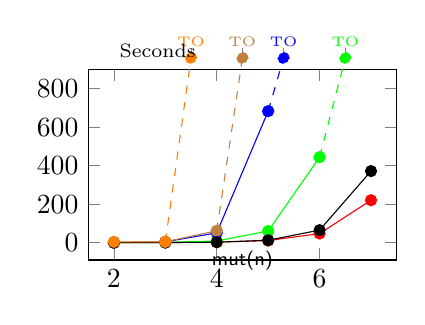
\begin{tikzpicture}
	\begin{axis}[name=Mutex,height=4cm,width=5.5cm,
		xlabel=\scriptsize{\textsf{mut(n)}},
		ylabel=\scriptsize{Seconds},
		x label style={at={(axis description cs:0.5,0.1)},anchor=north},
    	    y label style={at={(axis description cs:0.07,1.1)},anchor=west,rotate=-90},
    	%xmax=9,
		ymax=900,
		clip=false,
         %legend pos=north east
		]
    %exp2
	\addplot[color=red,mark=*] coordinates {
		(2, 0.461)
		(3, 0.877)
		(4, 2.945)
		(5, 11.05)
		(6, 47.634)
		(7, 220.863)
	};
	%exp4
	\addplot[color=green,mark=*] coordinates {
		(2, 0.483)
		(3, 1.602)
		(4, 9.032)
		(5, 60.845)
		(6, 444.691)
		%(6.5, 960) %time out
	};
	\addplot[color=green,mark=*,dashed] coordinates {		
		(6, 444.691)
		(6.5, 960) %time out
	}node[pin={[pin distance=-0.1cm]90:{\tiny{TO}}}]{};
	
	%exp8
	\addplot[color=blue,mark=*] coordinates {
		(2,0.983)
		(3,4.693)
		(4,51.233)
		(5,683.642)
		%(5.3,960) % time out
		%(7,1000)
		%(8,80.27)
		% (9,3600)
	};
	\addplot[color=blue,mark=*,dashed] coordinates {		
		(5,683.642)
		(5.3,960) % time out
		%(7,1000)
		%(8,80.27)
		% (9,3600)
	}node[pin={[pin distance=-0.1cm]90:{\tiny{TO}}}]{};
	
	%lineal10
	\addplot[color=brown,mark=*] coordinates {
		(2,0.608)
		(3,5.016)
		(4,62.034)
		%(4.5,960) % time out
		%(6,2.6)
		%(7,13.12)
		%(8,80.27)
		% (9,3600)
	};
	\addplot[color=brown,mark=*,dashed] coordinates {
		%(2,0.608)
		%(3,5.016)
		(4,62.034)
		(4.5,960) % time out
		%(6,2.6)
		%(7,13.12)
		%(8,80.27)
		% (9,3600)
	}node[pin={[pin distance=-0.1cm]90:{\tiny{TO}}}]{};
	%nocex
	\addplot[color=black,mark=*] coordinates {
		(2,0.348)
		(3,0.75)
		(4,2.679)
		(5,12.971)
		(6,65.403)
		(7,372.247)
		%(8,80.27)
		% (9,3600)
	};
	%psketch
	\addplot[color=orange,mark=*] coordinates {
		(2,4.62)
		(3,4.664)
		%(3.5,960)
		%(5,12.971)
		%(6,65.403)
		%(7,372.247)
		%(8,80.27)
		% (9,3600)
	};
	\addplot[color=orange,mark=*,dashed] coordinates {
		%(2,4.62)
		(3,4.664)
		(3.5,960)
		%(5,12.971)
		%(6,65.403)
		%(7,372.247)
		%(8,80.27)
		% (9,3600)
	}node[pin={[pin distance=-0.1cm]90:{\tiny{TO}}}]{};
	
	 %\addplot[color=black,mark=*] coordinates {
	% 	(9,3600)
	% } node[pin=180:{TO}]{};
	% \addplot[color=blue,dashed] coordinates {
	% 	(8,300)
	% 	(9,200)
	 %} node[pin=300:{TO}]{};
	%\addplot[color=green,mark=*,dashed] coordinates {
	%	(7,310)
		%(9, 107)
	%	} node[pin=180:{TO}]{};
	%\legend{exp2, exp4,exp8,lineal10,nocex}
	%\node[above right] at (rel axis cs:1, 1.1) {Time out:};
	%\node[above right] at (rel axis cs:0, 1) {\;\;\scriptsize{T.O:}};
	\end{axis}
\end{tikzpicture}
\label{fig:comparison}
% PHILOSOPHERS
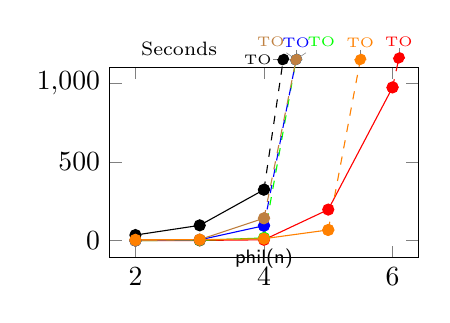
\begin{tikzpicture}
	\begin{axis}[name=Philosophers,height=4cm,width=5.5cm,
		xlabel=\scriptsize{\textsf{phil(n)}},
		ylabel=\scriptsize{Seconds},
		ymax=1100,
		clip=false,
		x label style={at={(axis description cs:0.5,0.1)},anchor=north},
    	y label style={at={(axis description cs:0.07,1.1)},anchor=west,rotate=-90},
		legend pos=north west]
    %exp2
	\addplot[color=red,mark=*] coordinates {
		(2,1.117)
		(3, 1.808)
		(4, 5.987)
		(5,197.652)
		(6,973.321)
		%(6.1,1160)
	};
	\addplot[color=red,mark=*,dashed] coordinates {
		(6,973.321)
		(6.1,1160)
	}node[pin={[pin distance=-0.1cm]90:{\tiny{TO}}}]{};
	%exp4
	\addplot[color=green,mark=*] coordinates {
		(2,1.253)
		(3, 2.765)
		(4, 17.661)
		%(4.5,1150)
		%(6,973.321)
		%(7,1000)
	};
	\addplot[color=green,mark=*,dashed] coordinates {
		(4, 17.661)
		(4.5,1150)
		%(6,973.321)
		%(7,1000)
	}node[pin={[pin distance=-0.1cm]60:{\tiny{TO}}}]{};
	
	%exp8
	\addplot[color=blue,mark=*] coordinates {
		(2,1.37)
		(3,5.552)
		(4,95.327)
		%(4.5,1150)
	     % (8,3600)
	};
	\addplot[color=blue,mark=*,dashed] coordinates {
		(4,95.327)
		(4.5,1150)
	     % (8,3600)
	}node[pin={[pin distance=-0.1cm]90:{\tiny{TO}}}]{};
	%lineal10
	\addplot[color=brown,mark=*] coordinates {
		(2,1.37)
		(3,7.264)
		(4,142.584)
		%(4.5,1150)
	     % (8,3600)
	};
	\addplot[color=brown,mark=*,dashed] coordinates {
		(4,142.584)
		(4.5,1150)
	     % (8,3600)
	}node[pin={[pin distance=-0.1cm]120:{\tiny{TO}}}]{};
	%nocex
	\addplot[color=black,mark=*] coordinates {
		(2,35.998)
		(3,97.636)
		(4,324)
		%(4.3,1150)
	     % (8,3600)
	};
	\addplot[color=black,mark=*,dashed] coordinates {
		(4,324)
		(4.3,1150)
	     % (8,3600)
	}node[pin={[pin distance=-0.1cm]180:{\tiny{TO}}}]{};
	%pskecth
	\addplot[color=orange,mark=*] coordinates {
		(2,5.916)
		(3,6.273)
		(4,12.845)%TO
		 (5,  68.5)
	     %(5.5,1150)
	};
	\addplot[color=orange,mark=*, dashed] coordinates {
		 (5,  68.5)
	     (5.5,1150)
	}node[pin={[pin distance=-0.1cm]90:{\tiny{TO}}}]{};
%\legend{exp2, PSketch}
     %\node[above right] at (rel axis cs:0, 1) {\;\;\scriptsize{T.O.:}};
	\end{axis}
\end{tikzpicture}
% BARRIER
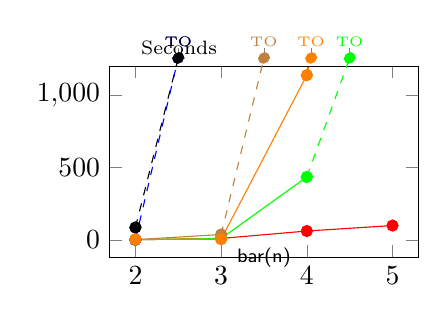
\begin{tikzpicture}
	\begin{axis}[name=SenseBarrier,height=4cm,width=5.5cm,
		xlabel=\scriptsize{\textsf{bar(n)}},
		ylabel=\scriptsize{Seconds},
		ymax=1200,
		clip=false,
		x label style={at={(axis description cs:0.5,0.1)},anchor=north},
    	y label style={at={(axis description cs:0.07,1.1)},anchor=west,rotate=-90},
		legend pos=north west]
    %exp2
	\addplot[color=red,mark=*] coordinates {
	    
		(2,1.535)
		(3, 10.761)
		(4, 62.111)
		(5,100)
		
	};
	%exp4
	\addplot[color=green,mark=*] coordinates {
	
		(2,1.672)
		(3, 10.569)
		(4, 436.365)
		%(4.5,1260) % TO
		%(6,973.321)
		%(7,1000)
	};
	\addplot[color=green,mark=*,dashed] coordinates {
		(4, 436.365)
		(4.5,1260) % TO
		%(6,973.321)
		%(7,1000)
	}node[pin={[pin distance=-0.1cm]90:{\tiny{TO}}}]{};
	
	%exp8
	\addplot[color=blue,mark=*] coordinates {
		(2,2.304)
	%	(2.5,1260)%TO
		%(4,95.327)
		%(5,1150)
	     % (8,3600)
	};
	\addplot[color=blue,mark=*,dashed] coordinates {
		(2,2.304)
		(2.5,1260)%TO
		%(4,95.327)
		%(5,1150)
	     % (8,3600)
	}node[pin={[pin distance=-0.1cm]90:{\tiny{TO}}}]{};
	%lineal10
	\addplot[color=brown,mark=*] coordinates {
	
		(2,2.362)
		(3,37.755)
		%(3.5,1260) % TO
		%(5,1150)
	     % (8,3600)
	};
	\addplot[color=brown,mark=*,dashed] coordinates {
	
		%(2,2.362)
		(3,37.755)
		(3.5,1260) % TO
		%(5,1150)
	     % (8,3600)
	}node[pin={[pin distance=-0.1cm]90:{\tiny{TO}}}]{};
	%nocex
	\addplot[color=black,mark=*] coordinates {
	   
		(2,86.916)
		%(2.5,1260)% TO
		%(4,324)
		%(4.3,1150)
	     % (8,3600)
	};
	\addplot[color=black,mark=*,dashed] coordinates {
	   
		(2,86.916)
		(2.5,1260)% TO
		%(4,324)
		%(4.3,1150)
	     % (8,3600)
	}node[pin={[pin distance=-0.1cm]90:{\tiny{TO}}}]{};
	%PSkecth
	\addplot[color=orange,mark=*] coordinates {
		(2,4.233)
		(3, 5.31)% TO
		(4,1140.9)
		%(4.05,1260)
	     % (8,3600)
	};
	\addplot[color=orange,mark=*,dashed] coordinates {
		(4,1140.9)
		(4.05,1260)
	     % (8,3600)
	}node[pin={[pin distance=-0.1cm]90:{\tiny{TO}}}]{};
%\legend{exp2, PSketch}
    %\node[above right] at (rel axis cs:0, 1) {\;\;\scriptsize{T.O.:}};
	\end{axis}
\end{tikzpicture}

% READERS & WRITERS
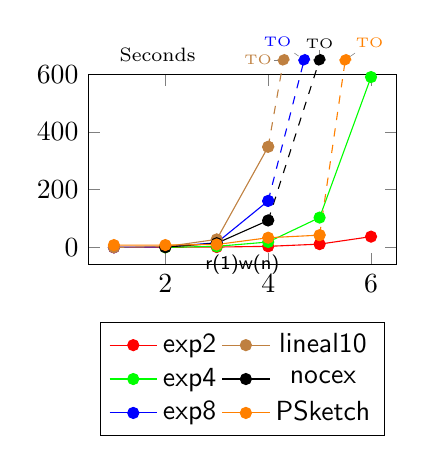
\begin{tikzpicture}
	\begin{axis}[name=Readers and Writers,height=4cm,width=5.5cm,
		xlabel=\scriptsize{\textsf{r(1)w(n)}},
		ylabel=\scriptsize{Seconds},
		x label style={at={(axis description cs:0.5,0.1)},anchor=north},
    	y label style={at={(axis description cs:0.07,1.1)},anchor=west,rotate=-90},
    	ymax=600,
		clip=false,
		legend style={at={(0.5,-0.3)},anchor=north,legend  columns =3, transpose legend}]
    % exp2
     \addlegendimage{red, line legend, mark=*} % or mark=none?
    \addlegendentry{\textsf{exp2}}
    \addlegendimage{green, line legend, , mark=*} % or mark=none?
    \addlegendentry{\textsf{exp4}}
    \addlegendimage{blue, line legend, , mark=*} % or mark=none?
    \addlegendentry{\textsf{exp8}}
    \addlegendimage{brown, line legend, , mark=*} % or mark=none?
    \addlegendentry{\textsf{lineal10}}
    \addlegendimage{black,,line legend,  mark=*} % or mark=none?
    \addlegendentry{\textsf{nocex}}
    \addlegendimage{orange,,line legend,  mark=*} % or mark=none?
    \addlegendentry{\textsf{PSketch}}
	\addplot[color=red,mark=*] coordinates {
		(1,0.492)
		(2,0.813)
		(3,1.603)
		(4,4.069)
		(5,11.705)
		(6,37.703)
	};
	% exp4
	\addplot[color=green,mark=*] coordinates {
		%(1,0.439)
		(2,0.442)
		(3,4.055)
		(4,19.064)
		(5,103.635)
		(6,590.277)
	};
	% exp8
	\addplot[color=blue,mark=*] coordinates {
		(1,0.625)
		(2,2.247)
		(3,16.51)
		(4,161.499)
		%(5,600) %TO
	};
	\addplot[color=blue,mark=*,dashed] coordinates {
		(4,161.499)
		(4.7,650) %TO
	}node[pin={[pin distance=-0.1cm]130:{\tiny{TO}}}]{};
	%lineal10
	\addplot[color=brown,mark=*] coordinates {
		(1,0.654)
		(2,2.892)
		(3,28.208)
		(4,348.931)
		%(4.3,660) %TO
	};
	\addplot[color=brown,mark=*,dashed] coordinates {
		(4,348.931)
		(4.3,650) %TO
	}node[pin={[pin distance=-0.1cm]180:{\tiny{TO}}}]{};
	\addplot[color=black,mark=*] coordinates {
		%(1,0.511)
		(2,1.344)
		(3,14.807)
		(4,93.844)
		%(5,600) %TO
	};
	\addplot[color=black,mark=*,dashed] coordinates {
		%(1,0.511)
		(4,93.844)
		(5,650) %TO
	}node[pin={[pin distance=-0.1cm]90:{\tiny{TO}}}]{};
	
	%PSketch
	\addplot[color=orange,mark=*] coordinates {
		(1,8.465)
		(2,8.483)
		(3,10.463)
		(4,33.898)
		(5,42.824)
		%(6,600)%TO
	};
	\addplot[color=orange,mark=*,dashed] coordinates {
		(5,42.824)
		(5.5,650)%TO
	}node[pin={[pin distance=-0.1cm]70:{\tiny{TO}}}]{};
   %\legend{exp2,exp4,exp8,lineal10,nocex,psketch}
    %\node[above right] at (rel axis cs:0, 1) {\;\;\scriptsize{T.O.:}};
	\end{axis}
\end{tikzpicture}
\vspace{0.4cm}
\captionof{figure}{Comparison between \\ \textsf{exp2}, \textsf{exp4}, \textsf{exp8},  \textsf{lineal10},  \textsf{nocex}, \\ and {\PSketch}.}
\label{fig:examples-plot}
\end{minipage}
\end{tabular}
\vspace{-0.5cm}
\end{table}
}
%{\scriptsize
%\begin{table}[!ht]
%\begin{tabular}{l l}
%\begin{minipage}{0.67\linewidth}
%    \centering
%    \begin{tabular}{|l|l|l|l|l|l|l|l|}
%    \hline
%        Ex. & Sc. & L.Time & G.Time & It. & R.St. & T.St. & Res. \\ \hline
%        Arb2 & 12 & 0.814 &  1.322 & 7 & $2^{2.32}$  & $2^{12}$ & F \\ \hline
%        Arb3 & 12 & 0.728 & 2.11 & 16 & $2^4$ & $2^18$ & F \\ \hline
%        Arb4 & 12 & 0.854 & 4.303 & 16 & $2^{5.24}$ & $2^{24}$ & F \\ \hline
%        Arb5 & 12 & 0.976 & 12.54 & 16 & $2^{6.35}$ & $2^{30}$ & F \\ \hline
%        Arb6 & 12 & 1.134 & 52.344 & 16 & $2^{7.40}$ & $2^{36}$ & F \\ \hline
%        FArb2 & 12 & 0.552 & 1.164 & 8 & $2^{2.58}$ & $2^{12}$ & F \\ \hline
%        FArb3 & 12 & 0.75 & 2.97 & 20 & $2^{3.45}$ & $2^{18}$ & F \\ \hline
%        FArb4 & 12 & 0.935 & 15.602 & 56 & $2^{4.39}$ & $2^{24}$ & F \\ \hline
%        FArb5 & 12 & 1.232 & 85.933 & 164 & $2^{5.35}$ & $2^{30}$ & F \\ \hline
%        FArb6 & 12 & 2.034 & 1004.49 & 857 & - & - & NF\\ \hline
%        FArb2 & 12 & 0.662 & 1.166 & 8 & $2^{2.80}$ & $2^{12}$ & F\\ \hline
%        PArb3 & 12 & 0.714 & 2.277 & 20 & $2^{3.45}$ & $2^{18}$ & F \\ \hline
%        PArb4 & 12 & 0.886 & 8.593 & 56 & $2^{4.39}$ & $2^{24}$ & F\\ \hline
%        PArb5 & 12 & 1.092 & 54.25 & 164 & $2^{5.35}$ & $2^{30}$ & F \\ \hline
%        PArb6 & 12 &1.324 & 700.731 & 488 & $2^{6.33}$ & $2^{36}$ & F \\ \hline
%    \end{tabular}
%\caption{Results for the Arbiter examples.}\label{tab:results-arbiter}
%\end{minipage}
%\begin{minipage}{0.50\linewidth}
%\centering
%\begin{tikzpicture}
%	\begin{axis}[name=Arbiter,height=4cm,width=5.5cm,
%		xlabel=\scriptsize{Arbiter(n)},
%		ylabel=\scriptsize{Seconds},
%		x label style={at={(axis description cs:0.5,0.1)},anchor=north},
%    	y label style={at={(axis description cs:0.07,1.1)},anchor=west,rotate=-90},
%    	ymax=75,
%		clip=false,
%		legend pos=north west]
%    % exp2
%	\addplot[color=red,mark=*] coordinates {
%		(2,0.768)
%		(3,1.563)
%		(4,2.175)
%		(5,3.768)
%		(6,9.172)
%		%(6,37.703)
%	};
%	% exp4
%	\addplot[color=green,mark=*] coordinates {
%		(2,0.78)
%		(3,1.687)
%		(4,3.085)
%		(5,6.985)
%		(6,19.659)
%	};
%	% exp8
%	\addplot[color=blue,mark=*] coordinates {
%		(2,0.67)
%		(3,2.132)
%		(4,4)
%		(5,10.624)
%		(6, 35.653) 
%	};
%	%lineal10
%	\addplot[color=brown,mark=*] coordinates {
%		(2,0.972)
%		(3,3.359)
%		(4,7.829)
%		(5,16.491)
%		(6,54.652)
%	};
%	%Party
%	\addplot[color=pink,mark=*] coordinates {
%		(2,0.63)
%		(3,1.18)
%		(4,2.82)
%		(5,6.12)
%		(6,12.43)
%	};
%	%nocex
%	%\addplot[color=black,mark=x] coordinates {
%	%	(1,0.511)
%	%	(2,1.344)
%	%	(3,14.807)
%	%	(4,93.844)
%	%	(5,600) %TO
%	%};
%	
%%\legend{exp2,exp4,exp8,lineal10,nocex}
%    \node[above right] at (rel axis cs:0, 1) {\;\;\scriptsize{Time out:}};
%	\end{axis}
%\end{tikzpicture}
%%Full Arbiter
%\begin{tikzpicture}
%	\begin{axis}[name=FullArbiter,height=4cm,width=5.5cm,
%		xlabel=\scriptsize{FullArbiter(n)},
%		ylabel=\scriptsize{Seconds},
%		x label style={at={(axis description cs:0.5,0.1)},anchor=north},
%    	y label style={at={(axis description cs:0.07,1.1)},anchor=west,rotate=-90},
%    	ymax=1200,
%		clip=false,
%		legend pos=north west]
%    % exp2
%	\addplot[color=red,mark=*] coordinates {
%		(2,1.164)
%		(3,2.97)
%		(4,15.609)
%		(5,85.933)
%		(6,1004.49)
%		%(6,37.703)
%	};
%	% exp4
%	\addplot[color=green,mark=*] coordinates {
%		(2,0.8)
%		(3,1.466)
%		(4,3.457)
%		(5,10.8)
%		(6,66.433)
%	};
%	% exp8
%	\addplot[color=blue,mark=*] coordinates {
%		(2,0.83)
%		(3,1.507)
%		(4,3.562)
%		(5,12.345)
%		(6, 69.144) %TO
%	};
%	%lineal10
%	\addplot[color=brown,mark=*] coordinates {
%		(2,2.024)
%		(3,19.822)
%		(4,298.955)
%		(5,1200)%TO
%	};
%	\addplot[color=pink,mark=*] coordinates {
%		(2,0.68)
%		(3,1.43)
%		(4,4.078)
%		(5,8.85)
%		(6,32.73)
%	};
%	%nocex
%	%\addplot[color=black,mark=x] coordinates {
%	%	(1,0.511)
%	%	(2,1.344)
%	%	(3,14.807)
%	%	(4,93.844)
%	%	(5,600) %TO
%	%};
%%\legend{exp2,exp4,exp8,lineal10,nocex}
%    \node[above right] at (rel axis cs:0, 1) {\;\;\scriptsize{Time out:}};
%	\end{axis}
%\end{tikzpicture}
%%PNUELIARBITER
%\begin{tikzpicture}
%	\begin{axis}[name=PnueliArbiter,height=4cm,width=5.5cm,
%		xlabel=\scriptsize{PnueliArbiter(n)},
%		ylabel=\scriptsize{Seconds},
%		x label style={at={(axis description cs:0.5,0.1)},anchor=north},
%    	y label style={at={(axis description cs:0.07,1.1)},anchor=west,rotate=-90},
%    	ymax=1400,
%		clip=false,
%		legend style={at={(0.2,-0.5)},anchor=north}]
%    % exp2
%	\addplot[color=red,mark=*] coordinates {
%		(2,1.168)
%		(3,2.277)
%		(4,8.593)
%		(5,54.25)
%		(6,1362.85) % TO
%		%(6,37.703)
%	};
%	% exp4
%	\addplot[color=green,mark=*] coordinates {
%		(2,0.676)
%		(3,1.146)
%		(4,2.355)
%		(5,11.6)
%		(6,66.433) 
%	};
%	% exp8
%	\addplot[color=blue,mark=*] coordinates {
%		(2,0.707)
%		(3,1.242)
%		(4,2.433)
%		(5,12.173)
%		(6, 65.155) %TO
%	};
%	%lineal10
%	\addplot[color=brown,mark=*] coordinates {
%		(2,0.69)
%		(3,1.162)
%		(4,2.408)
%		(5,11.836)
%		(6,59.299)
%	};
%	%nocex
%	%\addplot[color=black,mark=x] coordinates {
%	%	(1,0.511)
%	%	(2,1.344)
%	%	(3,14.807)
%	%	(4,93.844)
%	%	(5,600) %TO
%	%};
%	%party
%	\addplot[color=pink,mark=*] coordinates {
%		(2,0.69)
%		(3,1.162)
%		(4,2.408)
%		(5,11.836)
%		(6,1400)
%	};
%\legend{exp2,exp4,exp8,lineal10,nocex}
%    \node[above right] at (rel axis cs:0, 1) {\;\;\scriptsize{Time out:}};
%	\end{axis}
%\end{tikzpicture}
%\end{minipage}
%\end{tabular}
%\end{table}
%}

%\begin{figure}[hbt!]
%\begin{tabular}{l l}
%\begin{minipage}{0.48\linewidth}
%\centering
%%MUTEX
%\begin{tikzpicture}
%	\begin{axis}[name=Mutex,height=4cm,width=5.5cm,
%		xlabel=\scriptsize{Mutex(n)},
%		ylabel=\scriptsize{Seconds},
%		x label style={at={(axis description cs:0.5,0.1)},anchor=north},
%    	    y label style={at={(axis description cs:0.07,1.1)},anchor=west,rotate=-90},
%    	%xmax=9,
%		ymax=900,
%		clip=false,
%         %legend pos=north east
%		]
%    %exp2
%	\addplot[color=red,mark=*] coordinates {
%		(2, 0.461)
%		(3, 0.877)
%		(4, 2.945)
%		(5, 11.05)
%		(6, 47.634)
%		(7, 220.863)
%	};
%	%exp4
%	\addplot[color=green,mark=*] coordinates {
%		(2, 0.483)
%		(3, 1.602)
%		(4, 9.032)
%		(5, 60.845)
%		(6, 444.691)
%		(7, 900) %time out
%	};
%	%exp8
%	\addplot[color=blue,mark=*] coordinates {
%		(2,0.983)
%		(3,4.693)
%		(4,51.233)
%		(5,683.642)
%		(5.3,900) % time out
%		%(7,1000)
%		%(8,80.27)
%		% (9,3600)
%	};
%	%lineal10
%	\addplot[color=brown,mark=*] coordinates {
%		(2,0.608)
%		(3,5.016)
%		(4,62.034)
%		(5,900) % time out
%		%(6,2.6)
%		%(7,13.12)
%		%(8,80.27)
%		% (9,3600)
%	};
%	%nocex
%	\addplot[color=black,mark=*] coordinates {
%		(2,0.348)
%		(3,0.75)
%		(4,2.679)
%		(5,12.971)
%		(6,65.403)
%		(7,372.247)
%		%(8,80.27)
%		% (9,3600)
%	};
%	 %\addplot[color=black,mark=*] coordinates {
%	% 	(9,3600)
%	% } node[pin=180:{TO}]{};
%	% \addplot[color=blue,dashed] coordinates {
%	% 	(8,300)
%	% 	(9,200)
%	 %} node[pin=300:{TO}]{};
%	%\addplot[color=green,mark=*,dashed] coordinates {
%	%	(7,310)
%		%(9, 107)
%	%	} node[pin=180:{TO}]{};
%	%\legend{exp2, exp4,exp8,lineal10,nocex}
%	%\node[above right] at (rel axis cs:1, 1.1) {Time out:};
%	\node[above right] at (rel axis cs:0, 1) {\;\;\scriptsize{Time out:}};
%	\end{axis}
%\end{tikzpicture}
%\label{fig:comparison}
%% PHILOSOPHERS
%\begin{tikzpicture}
%	\begin{axis}[name=Philosophers,height=4cm,width=5.5cm,
%		xlabel=\scriptsize{Phils(n)},
%		ylabel=\scriptsize{Seconds},
%		ymax=1100,
%		clip=false,
%		x label style={at={(axis description cs:0.5,0.1)},anchor=north},
%    	y label style={at={(axis description cs:0.07,1.1)},anchor=west,rotate=-90},
%		legend pos=north west]
%    %exp2
%	\addplot[color=red,mark=*] coordinates {
%		(2,1.117)
%		(3, 1.808)
%		(4, 5.987)
%		(5,197.652)
%		(6,973.321)
%		(6.1,1100)
%	};
%	%exp4
%	\addplot[color=green,mark=*] coordinates {
%		(2,1.253)
%		(3, 2.765)
%		(4, 17.661)
%		(5,1100)
%		%(6,973.321)
%		%(7,1000)
%	};
%	%exp8
%	\addplot[color=blue,mark=*] coordinates {
%		(2,1.37)
%		(3,5.552)
%		(4,95.327)
%		(5,1100)
%	     % (8,3600)
%	};
%	%lineal10
%	\addplot[color=brown,mark=*] coordinates {
%		(2,1.37)
%		(3,7.264)
%		(4,142.584)
%		(5,1100)
%	     % (8,3600)
%	};
%	%nocex
%	\addplot[color=black,mark=*] coordinates {
%		(2,35.998)
%		(3,97.636)
%		(4,324)
%		(4.3,1100)
%	     % (8,3600)
%	};
%%\legend{exp2, PSketch}
%     \node[above right] at (rel axis cs:0, 1) {\;\;\scriptsize{Time out:}};
%	\end{axis}
%\end{tikzpicture}
%% BARRIER
%\begin{tikzpicture}
%	\begin{axis}[name=SenseBarrier,height=4cm,width=5.5cm,
%		xlabel=\scriptsize{SenseBarrier(n)},
%		ylabel=\scriptsize{Seconds},
%		ymax=500,
%		clip=false,
%		x label style={at={(axis description cs:0.5,0.1)},anchor=north},
%    	y label style={at={(axis description cs:0.07,1.1)},anchor=west,rotate=-90},
%		legend pos=north west]
%    %exp2
%	\addplot[color=red,mark=*] coordinates {
%	    
%		(2,1.535)
%		(3, 10.761)
%		(4, 62.111)
%		(5,100)
%		
%	};
%	%exp4
%	\addplot[color=green,mark=*] coordinates {
%	
%		(2,1.672)
%		(3, 10.569)
%		(4, 436.365)
%		(4.1,500) % TO
%		%(6,973.321)
%		%(7,1000)
%	};
%	%exp8
%	\addplot[color=blue,mark=*] coordinates {
%	
%		(2,2.304)
%		(3,500)%TO
%		%(4,95.327)
%		%(5,1150)
%	     % (8,3600)
%	};
%	%lineal10
%	\addplot[color=brown,mark=*] coordinates {
%	
%		(2,2.362)
%		(3,37.755)
%		(4,500) % TO
%		%(5,1150)
%	     % (8,3600)
%	};
%	%nocex
%	\addplot[color=black,mark=*] coordinates {
%	   
%		(2,86.916)
%		(2.5,500)% TO
%		%(4,324)
%		%(4.3,1150)
%	     % (8,3600)
%	};
%%\legend{exp2, PSketch}
%    \node[above right] at (rel axis cs:0, 1) {\;\;\scriptsize{Time out:}};
%	\end{axis}
%\end{tikzpicture}
%
%% READERS & WRITERS
%\begin{tikzpicture}
%	\begin{axis}[name=Readers and Writers,height=4cm,width=5.5cm,
%		xlabel=\scriptsize{RW(1,n)},
%		ylabel=\scriptsize{Seconds},
%		x label style={at={(axis description cs:0.5,0.1)},anchor=north},
%    	y label style={at={(axis description cs:0.07,1.1)},anchor=west,rotate=-90},
%    	ymax=600,
%		clip=false,
%		legend pos=north west]
%    % exp2
%	\addplot[color=red,mark=*] coordinates {
%		(1,0.492)
%		(2,0.813)
%		(3,1.603)
%		(4,4.069)
%		(5,11.705)
%		(6,37.703)
%	};
%	% exp4
%	\addplot[color=green,mark=*] coordinates {
%		(1,0.439)
%		(2,0.442)
%		(3,4.055)
%		(4,19.064)
%		(5,103.635)
%		(6,590.277)
%	};
%	% exp8
%	\addplot[color=blue,mark=*] coordinates {
%		(1,0.625)
%		(2,2.247)
%		(3,16.51)
%		(4,161.499)
%		(5,600) %TO
%	};
%	%lineal10
%	\addplot[color=brown,mark=*] coordinates {
%		(1,0.654)
%		(2,2.892)
%		(3,28.208)
%		(4,348.931)
%		(4.3,600) %TO
%	};
%	\addplot[color=black,mark=*] coordinates {
%		(1,0.511)
%		(2,1.344)
%		(3,14.807)
%		(4,93.844)
%		(5,600) %TO
%	};
%
%%\legend{exp2,exp4,exp8,lineal10,nocex}
%    \node[above right] at (rel axis cs:0, 1) {\;\;\scriptsize{Time out:}};
%	\end{axis}
%\end{tikzpicture}
%\end{minipage}
%%\captionof{figure}{Comparison for exp2, exp4, exp8, lineal10, and nocex.}
%&
%%%% ARBITER EXAMPLES
%%Arbiter
%\begin{minipage}{0.48\linewidth}
%\centering
%\begin{tikzpicture}
%	\begin{axis}[name=Arbiter,height=4cm,width=5.5cm,
%		xlabel=\scriptsize{Arbiter(n)},
%		ylabel=\scriptsize{Seconds},
%		x label style={at={(axis description cs:0.5,0.1)},anchor=north},
%    	y label style={at={(axis description cs:0.07,1.1)},anchor=west,rotate=-90},
%    	ymax=75,
%		clip=false,
%		legend pos=north west]
%    % exp2
%	\addplot[color=red,mark=*] coordinates {
%		(2,0.768)
%		(3,1.563)
%		(4,2.175)
%		(5,3.768)
%		(6,9.172)
%		%(6,37.703)
%	};
%	% exp4
%	\addplot[color=green,mark=*] coordinates {
%		(2,0.78)
%		(3,1.687)
%		(4,3.085)
%		(5,6.985)
%		(6,19.659)
%	};
%	% exp8
%	\addplot[color=blue,mark=*] coordinates {
%		(2,0.67)
%		(3,2.132)
%		(4,4)
%		(5,10.624)
%		(6, 35.653) 
%	};
%	%lineal10
%	\addplot[color=brown,mark=*] coordinates {
%		(2,0.972)
%		(3,3.359)
%		(4,7.829)
%		(5,16.491)
%		(6,54.652)
%	};
%	%Party
%	\addplot[color=pink,mark=*] coordinates {
%		(2,0.63)
%		(3,1.18)
%		(4,2.82)
%		(5,6.12)
%		(6,12.43)
%	};
%	%nocex
%	%\addplot[color=black,mark=x] coordinates {
%	%	(1,0.511)
%	%	(2,1.344)
%	%	(3,14.807)
%	%	(4,93.844)
%	%	(5,600) %TO
%	%};
%	
%%\legend{exp2,exp4,exp8,lineal10,nocex}
%    \node[above right] at (rel axis cs:0, 1) {\;\;\scriptsize{Time out:}};
%	\end{axis}
%\end{tikzpicture}
%%Full Arbiter
%\begin{tikzpicture}
%	\begin{axis}[name=FullArbiter,height=4cm,width=5.5cm,
%		xlabel=\scriptsize{FullArbiter(n)},
%		ylabel=\scriptsize{Seconds},
%		x label style={at={(axis description cs:0.5,0.1)},anchor=north},
%    	y label style={at={(axis description cs:0.07,1.1)},anchor=west,rotate=-90},
%    	ymax=1200,
%		clip=false,
%		legend pos=north west]
%    % exp2
%	\addplot[color=red,mark=*] coordinates {
%		(2,1.164)
%		(3,2.97)
%		(4,15.609)
%		(5,85.933)
%		(6,1004.49)
%		%(6,37.703)
%	};
%	% exp4
%	\addplot[color=green,mark=*] coordinates {
%		(2,0.8)
%		(3,1.466)
%		(4,3.457)
%		(5,10.8)
%		(6,66.433)
%	};
%	% exp8
%	\addplot[color=blue,mark=*] coordinates {
%		(2,0.83)
%		(3,1.507)
%		(4,3.562)
%		(5,12.345)
%		(6, 69.144) %TO
%	};
%	%lineal10
%	\addplot[color=brown,mark=*] coordinates {
%		(2,2.024)
%		(3,19.822)
%		(4,298.955)
%		(5,1200)%TO
%	};
%	\addplot[color=pink,mark=*] coordinates {
%		(2,0.68)
%		(3,1.43)
%		(4,4.078)
%		(5,8.85)
%		(6,32.73)
%	};
%	%nocex
%	%\addplot[color=black,mark=x] coordinates {
%	%	(1,0.511)
%	%	(2,1.344)
%	%	(3,14.807)
%	%	(4,93.844)
%	%	(5,600) %TO
%	%};
%%\legend{exp2,exp4,exp8,lineal10,nocex}
%    \node[above right] at (rel axis cs:0, 1) {\;\;\scriptsize{Time out:}};
%	\end{axis}
%\end{tikzpicture}
%%PNUELIARBITER
%\begin{tikzpicture}
%	\begin{axis}[name=PnueliArbiter,height=4cm,width=5.5cm,
%		xlabel=\scriptsize{PnueliArbiter(n)},
%		ylabel=\scriptsize{Seconds},
%		x label style={at={(axis description cs:0.5,0.1)},anchor=north},
%    	y label style={at={(axis description cs:0.07,1.1)},anchor=west,rotate=-90},
%    	ymax=1400,
%		clip=false,
%		legend style={at={(0.2,-0.5)},anchor=north}]
%    % exp2
%	\addplot[color=red,mark=*] coordinates {
%		(2,1.168)
%		(3,2.277)
%		(4,8.593)
%		(5,54.25)
%		(6,1362.85) % TO
%		%(6,37.703)
%	};
%	% exp4
%	\addplot[color=green,mark=*] coordinates {
%		(2,0.676)
%		(3,1.146)
%		(4,2.355)
%		(5,11.6)
%		(6,66.433) 
%	};
%	% exp8
%	\addplot[color=blue,mark=*] coordinates {
%		(2,0.707)
%		(3,1.242)
%		(4,2.433)
%		(5,12.173)
%		(6, 65.155) %TO
%	};
%	%lineal10
%	\addplot[color=brown,mark=*] coordinates {
%		(2,0.69)
%		(3,1.162)
%		(4,2.408)
%		(5,11.836)
%		(6,59.299)
%	};
%	%nocex
%	%\addplot[color=black,mark=x] coordinates {
%	%	(1,0.511)
%	%	(2,1.344)
%	%	(3,14.807)
%	%	(4,93.844)
%	%	(5,600) %TO
%	%};
%	%party
%	\addplot[color=pink,mark=*] coordinates {
%		(2,0.69)
%		(3,1.162)
%		(4,2.408)
%		(5,11.836)
%		(6,1400)
%	};
%\legend{exp2,exp4,exp8,lineal10,nocex}
%    \node[above right] at (rel axis cs:0, 1) {\;\;\scriptsize{Time out:}};
%	\end{axis}
%\end{tikzpicture}
%\vspace{1.3cm}
%
%%\captionof{figure}{Comparison with Party Tool.}
%\label{fig:comparison}
%\end{minipage}
%\end{tabular}
%\end{figure}
We evaluate our approach around the following research questions: 
\begin{description}
\item[RQ1] \emph{How effective/efficient is our synthesis approach?}
\item[RQ2] \emph{How good is the counterexample-guided search for speeding up the synthesis method?}
\item[RQ3] \emph{How do the selected bounds affect the synthesis method?}
\item[RQ4] \emph{How does our approach compare with related approaches?}
\end{description}
To answer these questions,  we implemented Alg.~\ref{alg:improved_alg} in a prototype tool, it uses the \textsf{Alloy Analyzer}~\cite{AlloyBook} for obtaining instances of specifications, and {\NuSMV}~\cite{Cimatti+2002} for model checking the candidates.  We evaluate our approach on eight  examples of distributed algorithms: the dining philosophers (\textsf{phil})~\cite{Dijkstra71} (our running example), Mutex (\textsf{mut})~\cite{Fokkink13},  Readers and Writers (\textsf{rw})~\cite{Fokkink13}, the generalized version of Peterson's algorithm (\textsf{pet})~\cite{Fokkink13},   and the combined-tree Barrier protocol (\textsf{bar})~\cite{Fokkink13}.  Furthermore,  we  also encoded the arbiter examples presented in \cite{Party,Piterman+2006}: a simple arbiter (\textsf{arb}), a full arbiter (\textsf{farb}), and the Pnueli arbiter (\textsf{parb}). These case studies assume a distributed token ring architecture,  which we modeled using the Alloy language.  

%\cite{PhilStone}. The tool takes as input a  specification and returns, when possible, an LTS satisfying the specification, described in the \NuSMV  language.
Tables~\ref{tab:results-common} and~\ref{tab:results-arbiter}  summarize the experimental results. The experiments were conducted on an Apple M2 processor with 16GB of memory.   In these examples, we used the sequence of bounds $2,4,8,16,\dots$, named \textsf{exp2} from now on.
For each case study, we report the 
bound over the size of the processes (Sc), the maximum time needed to generate local process instances (L.Time), the total time required for synthesizing the system (T.Time), the number of times that the model checker was invoked (Its) by the synthesizer, and the final result of our synthesis algorithm:  `F' (if an implementation was found),  `N'  (if no implementation was found),  `TO'  if the example timed out, or `U'  (if the specification was found unsatisfiable by the Alloy tool).  We also report the number of reachable states (R.St.), and the total states (T.St.) of the obtained implementations, expressed as power of $2$.  For space reasons, we only include a few configurations found unsatisfiable by the solver; similar numbers can be obtained for the rest of the cases if the specifications are processed with smaller scopes. We also indicate the number of processes considered in each experiment.  For instance,  \textsf{phil(6)} indicates that we considered \textsf{6} concurrent processes (i.e., philosophers) in the dining philosophers example. In the case of Readers and Writers, 
\textsf{r(n)w(m)} means that \textsf{n} readers and \textsf{m} writers were considered.  We  have  set out a time out of 30 minutes.
\begin{wraptable}[19]{r}{.60\textwidth}
\vspace{-0.5cm}
\begin{tabular}{|l|l|l|l|l|l|l|l|}
    \hline
        Ex. & Sc. & L.Time & G.Time & It. & R.St. & T.St. & Res. \\ \hline
        \textsf{arb(2)} & 12 & 0.814 &  1.322 & 7 & $2^{2.32}$  & $2^{12}$ & F \\ \hline
        \textsf{arb(3)} & 12 & 0.728 & 2.11 & 16 & $2^4$ & $2^{18}$ & F \\ \hline
        \textsf{arb(4)} & 12 & 0.854 & 4.303 & 16 & $2^{5.24}$ & $2^{24}$ & F \\ \hline
        \textsf{arb(5)} & 12 & 0.976 & 12.54 & 16 & $2^{6.35}$ & $2^{30}$ & F \\ \hline
        \textsf{arb(6)} & 12 & 1.134 & 52.344 & 16 & $2^{7.40}$ & $2^{36}$ & F \\ \hline
        \textsf{farb(2)} & 12 & 0.552 & 1.164 & 8 & $2^{2.58}$ & $2^{12}$ & F \\ \hline
        \textsf{farb(3)} & 12 & 0.75 & 2.97 & 20 & $2^{3.45}$ & $2^{18}$ & F \\ \hline
        \textsf{farb(4)} & 12 & 0.935 & 15.602 & 56 & $2^{4.39}$ & $2^{24}$ & F \\ \hline
        \textsf{farb(5)} & 12 & 1.232 & 85.933 & 164 & $2^{5.35}$ & $2^{30}$ & F \\ \hline
        \textsf{farb(6)} & 12 & 2.034 & 672.539 & 488 & $2^{6.33}$ & $2^{36}$ & F\\ \hline
        \textsf{parb(2)} & 12 & 0.662 & 1.166 & 8 & $2^{2.80}$ & $2^{12}$ & F\\ \hline
        \textsf{parb(3)} & 12 & 0.714 & 2.277 & 20 & $2^{3.45}$ & $2^{18}$ & F \\ \hline
        \textsf{parb(4)} & 12 & 0.886 & 8.593 & 56 & $2^{4.39}$ & $2^{24}$ & F\\ \hline
        \textsf{parb(5)} & 12 & 1.092 & 54.25 & 164 & $2^{5.35}$ & $2^{30}$ & F \\ \hline
        \textsf{parb(6)} & 12 &1.324 & 700.731 & 488 & $2^{6.33}$ & $2^{36}$ & F \\ \hline
\end{tabular}
\caption{Results for the arbiter examples.}\label{tab:results-arbiter}
\end{wraptable}
%
Table \ref{tab:results-common} shows that the technique scales reasonably well for those case studies in which each process uses only a reduced number of locks and shared variables (e.g., dining philosophers, mutex and reader-writers). For the cases where the number of shared variables accessed by the processes is bigger (e.g., Peterson for $n$ processes), the technique does not scale that well. Intuitively, more shared variables imply more actions performed by the environment, which increases the size of the formula fed to the SAT solver.  We plan to investigate how to equip specifications with assumptions on the environment's behavior, to restrict the possible values of shared variables; this may simplify the SAT problem when searching for local implementations.  It is worth noting, that even though the algorithm is incomplete, we have not 
observed any ``not found'' outputs in our benchmarks. This could be due to  the set timeouts.  We leave an in-depth investigation of this as further work.

 To answer \textbf{RQ3}   we compare the results obtained with several configurations of bounds for the exploration phase, namely: \textsf{exp4} ($4,16,64,\dots$),  \textsf{exp8} ($8,64,512,\dots$),  \textsf{lineal10} ($10,20,30,\dots$), and for \textbf{RQ2} we also considered Alg.~\ref{alg:the_alg},  which does not take into account counterexamples (\textsf{nocex}).  The obtained results are depicted in Figs.\ref{fig:examples-plot} and \ref{fig:arbiter-plots}.  Note that time outs are remarked using dashed lines going out of the $y$-axis.
 In general, \textsf{exp2} behaves better than the other options,  thus it seems better to collect a few counterexamples first, and use them to improve the search.  A possible drawback of this setting is that a wrong choice of the first counterexamples may have as a consequence that no implementation is found,  i.e., one may expect that this configuration  is ``more incomplete''   than the other options. However, we have not observed this in our benchmarks.  Note that \textsf{nocex} timed out in many examples. Indeed, for the arbiter examples, \textsf{nocex} was able only to solve the examples with two processes,  taking for that more than $7000$ iterations.

\begin{wrapfigure}[31]{hr}{.40\textwidth}
\vspace{-1.5cm}
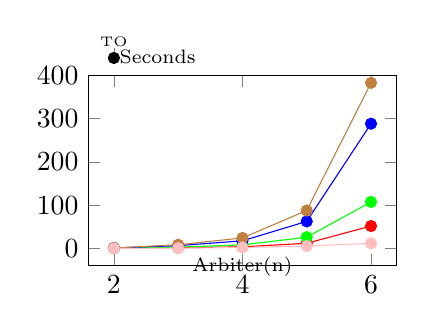
\begin{tikzpicture}
	\begin{axis}[name=Arbiter,height=4cm,width=5.5cm,
		xlabel=\scriptsize{Arbiter(n)},
		ylabel=\scriptsize{Seconds},
		x label style={at={(axis description cs:0.5,0.1)},anchor=north},
    	y label style={at={(axis description cs:0.07,1.1)},anchor=west,rotate=-90},
    	ymax=400,
		clip=false,
		legend pos=north west]
    % exp2
	\addplot[color=red,mark=*] coordinates {
		(2,1.3)
		(3,2.11)
		(4,4.3)
		(5,12.54)
		(6,52.34)
		%(6,37.703)
	};
	% exp4
	\addplot[color=green,mark=*] coordinates {
		(2,1.372)
		(3,3.545)
		(4,8.824)
		(5,26.531)
		(6,107.897)
	};
	% exp8
	\addplot[color=blue,mark=*] coordinates {
		(2,1.72)
		(3,7.022)
		(4,18.176)
		(5,63.028)
		(6, 288.419) 
	};
	%lineal10
	\addplot[color=brown,mark=*] coordinates {
		(2,1.737)
		(3,9.11)
		(4,24.866)
		(5,88.064)
		(6,382.565)
	};
	%Party
	\addplot[color=pink,mark=*] coordinates {
		(2,0.63)
		(3,1.18)
		(4,2.82)
		(5,6.12)
		(6,12.43)
	};
	%nocex
	\addplot[color=black,mark=*] coordinates {
	%	(1,0.511)
		(2,440)
	%	(3,14.807)
	%	(4,93.844)
	%	(5,600) %TO
	}node[pin={[pin distance=-0.1cm]90:{\tiny{TO}}}]{};

%\legend{exp2,exp4,exp8,lineal10,nocex}
    %\node[above right] at (rel axis cs:0, 1) {\;\;\scriptsize{T.O.:}};
	\end{axis}
\end{tikzpicture}
%Full Arbiter
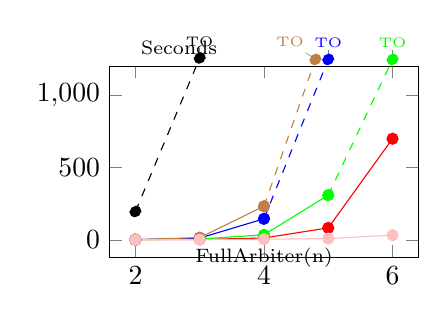
\begin{tikzpicture}
	\begin{axis}[name=FullArbiter,height=4cm,width=5.5cm,
		xlabel=\scriptsize{FullArbiter(n)},
		ylabel=\scriptsize{Seconds},
		x label style={at={(axis description cs:0.5,0.1)},anchor=north},
    	y label style={at={(axis description cs:0.07,1.1)},anchor=west,rotate=-90},
    	ymax=1200,
		clip=false,
		legend pos=north west]
    % exp2
	\addplot[color=red,mark=*] coordinates {
		(2,1.083)
		(3,2.774)
		(4,12.873)
		(5,82.981)
		(6,700.731)
		%(6,37.703)
	};
	% exp4
	\addplot[color=green,mark=*] coordinates {
		(2,1.24)
		(3,5.719)
		(4,34.7)
		(5,309.953)
	};
	\addplot[color=green,mark=*,dashed] coordinates {
		(5,309.953)
		(6,1250)
	}node[pin={[pin distance=-0.1cm]90:{\tiny{TO}}}]{};
	
	% exp8
	\addplot[color=blue,mark=*] coordinates {
		(2,1.55)
		(3,12.382)
		(4,145.86)
	};
	\addplot[color=blue,mark=*,dashed] coordinates {
		(4,145.86)
		(5,1250)
	}node[pin={[pin distance=-0.1cm]90:{\tiny{TO}}}]{};
	
	%lineal10
	\addplot[color=brown,mark=*] coordinates {
		(2,1.677)
		(3,15.45)
		(4,232.942)
		%(5,1250)%TO
	};
	\addplot[color=brown,mark=*,dashed] coordinates {
		(4,232.942)
		(4.8,1250)%TO
	}node[pin={[pin distance=-0.1cm]120:{\tiny{TO}}}]{};
	    
	%Party
	\addplot[color=pink,mark=*] coordinates {
		(2,0.68)
		(3,1.43)
		(4,4.078)
		(5,8.85)
		(6,32.73)
	};
	%nocex
	\addplot[color=black,mark=*,dashed] coordinates {
	%	(1,0.511)
		(2,196.115)
		(3,1260) % TO
	%	(4,93.844)
	%	(5,600) %TO
	}node[pin={[pin distance=-0.1cm]90:{\tiny{TO}}}]{};
	
%\legend{exp2,exp4,exp8,lineal10,nocex}
    %\node[above right] at (rel axis cs:0, 1) {\;\;\scriptsize{T.O.:}};
	\end{axis}
\end{tikzpicture}
%PNUELIARBITER
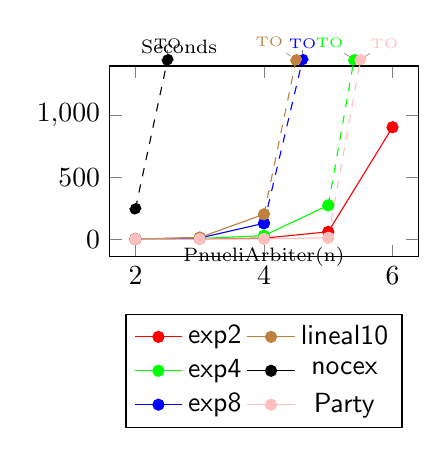
\begin{tikzpicture}
	\begin{axis}[name=PnueliArbiter,height=4cm,width=5.5cm,
		xlabel=\scriptsize{PnueliArbiter(n)},
		ylabel=\scriptsize{Seconds},
		x label style={at={(axis description cs:0.5,0.1)},anchor=north},
    	y label style={at={(axis description cs:0.07,1.1)},anchor=west,rotate=-90},
    	ymax=1400,
		clip=false,
		legend style={at={(0.5,-0.3)},anchor=north,legend  columns =3, transpose legend}]
    % exp2
     \addlegendimage{red, line legend, mark=*} % or mark=none?
    \addlegendentry{\textsf{exp2}}
    \addlegendimage{green, line legend, , mark=*} % or mark=none?
    \addlegendentry{\textsf{exp4}}
    \addlegendimage{blue, line legend, , mark=*} % or mark=none?
    \addlegendentry{\textsf{exp8}}
    \addlegendimage{brown, line legend, , mark=*} % or mark=none?
    \addlegendentry{\textsf{lineal10}}
    \addlegendimage{black,,line legend,  mark=*} % or mark=none?
    \addlegendentry{\textsf{nocex}}
    \addlegendimage{pink,line legend,  mark=*} % or mark=none?
    \addlegendentry{\textsf{Party}}
    % exp2
	\addplot[color=red,mark=*] coordinates {
		(2,1.206)
		(3,2.674)
		(4,8.639)
		(5,59.893)
		(6,905.203) % TO
		%(6,37.703)
	};
	% exp4
	\addplot[color=green,mark=*] coordinates {
		(2,1.406)
		(3,5.461)
		(4,29.063)
		(5,274.013)
	};
	\addplot[color=green,mark=*,dashed] coordinates {
		(5,274.013)
		(5.4,1450) 
	}node[pin={[pin distance=-0.1cm]110:{\tiny{TO}}}]{};
	
	% exp8
	\addplot[color=blue,mark=*] coordinates {
		(2,1.634)
		(3,9.749)
		(4,128.565)
	};
	\addplot[color=blue,mark=*,dashed] coordinates {
		(4,128.565)
		(4.6, 1450) %TO
	}node[pin={[pin distance=-0.1cm]90:{\tiny{TO}}}]{};
	%lineal10
	\addplot[color=brown,mark=*] coordinates {
		(2,1.789)
		(3,13.855)
		(4,201.653)
	};
	\addplot[color=brown,mark=*,dashed] coordinates {	
		(4,201.653)
		(4.5,1450)
	}node[pin={[pin distance=-0.1cm]130:{\tiny{TO}}}]{};
	%nocex
	\addplot[color=black,mark=*,dashed] coordinates {
	%	(1,0.511)
		(2,246.157)
	 	(2.5,1450)
	%	(4,93.844)
	%	(5,600) %TO
	}node[pin={[pin distance=-0.1cm]90:{\tiny{TO}}}]{};
	%party
	\addplot[color=pink,mark=*] coordinates {
		(2,0.69)
		(3,1.162)
		(4,2.408)
		(5,11.836)
		%(5.5,1450)
	};
	\addplot[color=pink,mark=*,dashed] coordinates {
		(5,11.836)
		(5.5,1450)
	}node[pin={[pin distance=-0.1cm]80:{\tiny{TO}}}]{};
    %\legend{exp2,exp4,exp8,lineal10,nocex,Party}
    %\node[above right] at (rel axis cs:0, 1) {\;\;\scriptsize{T.O.:}};
	\end{axis}
\end{tikzpicture}
\caption{Efficiency comparison for arbiter examples}\label{fig:arbiter-plots}
\end{wrapfigure}
To answer \textbf{RQ4} we have included in out analysis the synthesis tool {\PSketch}~\cite{Solar-Lezama+2008}, that implements a Counterexample-driven Guided Inductive Synthesis (CEGIS) algorithm to obtain code from sketched code (i.e., code annotated with ``holes''). To run {\PSketch}, we took the Dining Philosophers specification provided in~\cite{Solar-Lezama+2008}, and manually elaborated the specification for Mutex,  Readers-Writers, and the Barrier example.  The Peterson example cannot be analysed with  {\PSketch} since this tool only supports the analysis of safety properties.  For the arbiter case studies, we have compare against the tool {\Party} \cite{Party} which is a tool specifically tailored for distributed systems that use token ring architectures.

Our comparison focuses only on the time required by each technique for synthesizing the distributed solutions. The plots of Figs.~\ref{fig:examples-plot} and \ref{fig:arbiter-plots} depict the results of this comparison. In all the case studies, we notice that the efficiency of {\PSketch} is drastically affected as the number of processes to synthesize is incremented. For instance, in the dining philosophers with 6 processes, {\Sketch} timed out; in contrast, our tool was able to obtain a solution. Similarly, in the case of 1 reader and 6 writers, {\PSketch} failed in synthesizing a solution, while our approach succeeded. A similar analysis applies to Mutex.

  In the case of the tool {\Party}, for the \textsf{arb} and \textsf{farb} examples {\Party} was able to find solutions faster than \textsf{exp2}; it must be noted that in these cases {\Party} uses a cut-off of $4$,  i.e., it reduces configurations with $n>4$ processes to the case $n=4$.  However,  even though {\Party} has several optimizations for token ring systems, our tool was able to synthesize an implementation of the \textsf{parb(6)} and {\Party} timed out for this case. 
  
It is worth noting that the tool can be used to find different solutions for some examples.  We have experimented with this using the \textsf{phil} example, where, after finding an initial solution, we allow the algorithm to keep looking for further solutions, and it succeeded in finding a second solution.  For space reasons we do not investigate this aspect of the tool further here.

%For instance, for the dining philosophers, the first found solution is one in which each philosopher takes a fork only if her two forks are available (a know solution to prevent deadlock). When we allow the algorithm to keep looking for further solutions, it succeeded in finding a second solution, the ``even/odd'' solution, where $n-1$ philosophers take first their left fork and after their right fork, whereas  philosopher $n$ takes first her right fork and then her left fork.  

\section{Discussion and Future Work}\label{sec:discussion}
This paper pioneers the novel approach of selective response, showing that withholding responses can be a powerful tool for GenAI systems. By opting not to answer every query as accurately as it can---particularly when new or complex topics emerge---GenAI can encourage user participation on community-driven platforms and thereby generate more high-quality data for future training. This mechanism ultimately enhances GenAI's long-term performance and revenue. From a welfare perspective, our results indicate that such selective engagement can also benefit users, leading to better solutions and increased overall satisfaction. Since this work is the first to address selective response strategies for GenAI, numerous promising directions remain for future research; we highlight some of them below. 

First, from a technical standpoint, all of the results in this paper rely on Assumption~\ref{assumption: data lip}, involving the lipshitz condition of the accuracy function and the sensitivity parameter $\beta$. Future work could seek to relax this assumption. Furthermore, our constrained optimization approach in Subsection~\ref{sec: welfare constrained revenue maximization} could be extended to approximate the optimal (continuous) strategy instead of the optimal discrete strategy.

Second, our stylized model adopts the simplifying---though unrealistic---assumption that only a single GenAI platform exists. Admittedly, this makes it easier to focus on the idea of selective responses, and indeed, this assumption is pivotal in keeping our analysis tractable. Future research could explore scenarios with multiple GenAI platforms and human-centered forums. In such settings, one platform's selective response might redirect users not only to forums but also to competing GenAI platforms, leading to the tragedy of the commons \cite{hardin1968tragedy}: Although all GenAI platforms benefit from fresh data generation, none may choose to respond selectively if it means losing users to competitors. 

Third, we assumed Forum behaves non-strategically. In reality, human-centered platforms often monetize their data by selling it to GenAI platforms, adding a further layer of strategic interaction for GenAI. Moreover, data transfer between the platforms can form the basis for collaboration: GenAI could employ selective response to bolster Forum content creation, and Forum could, in turn, attribute that content to GenAI for subsequent use in retraining.


%Third, we make the (again) simplifying assumption that Forum is non-strategic. However, in practice, human-centered platforms can sell their data to GenAI platforms. This adds additional considerations for GenAI. Furthermore, data transmission between the platforms can also become the basis for collaboration: GenAI can use selective response to ensure enough content is generated in Forum, and Forum could provide the data attributed to this mechanism back to GenAI. 


%Second, this paper makes the simplifying yet unrealistic assumption of the existence of one GenAI platform. Indeed, this simplifies many aspects and allows us to analyze selective responses. Future work could address the data generation process with more than one GenAI platform and possibly several human-centered forums. In such a case, selective response of one GenAI platform can either drive users to forums or to other GenAI platforms; thus, we might face a tragedy of the commons situation~\ref{hardin1968tragedy}, where all GenAI platforms are interested in fresh data generation but none volunteer to selectively respond and lose users. 

%This paper examines the competition between a generative AI platform and human-based platforms, challenging the assumption that always providing answers is optimal. We analyzed the impact of withholding answers on GenAI's revenue and developed an efficient approximately optimal algorithm for this purpose. We further explored how withholding affects users, showing that it can lead to better outcomes compared to always answering. Specifically, we demonstrated that withholding can Pareto-dominate this strategy and derived the necessary and sufficient conditions for that. Finally, we proposed a second approximately optimal algorithm that maximizes GenAI's revenue while ensuring users are better off than when GenAI answers all queries.

%On a more conceptual level, our model assumes that GenAI’s data comes solely from the competing platform (Forum). Future research could explore a scenario where GenAI can purchase additional data from a third party. This extension could provide valuable insights into the interplay between withholding answers and data purchasing, and whether these two strategies can complement each other or must be traded off.


\acks{This work was supported by the ERC grant \#786854 G-Statistics from the European Research Council under the European Union’s Horizon 2020 research and innovation program and by the French government through the 3IA Côte d’Azur Investments ANR-19-P3IA-0002 managed by the National Research Agency.}

\newpage

\appendix
\subsection{The flag trick for robust subspace recovery problems}
Let us consider a dataset that is a union of \textit{inliers} and \textit{outliers}---the inliers are assumed to lie near a low-dimensional subspace $\S$ while the outliers live in the ambient space. The aim of robust subspace recovery (RSR) is to recover $\S$~\citep{lerman_overview_2018}. In that sense, RSR is an outlier-robust extension of classical dimension reduction methods like PCA.
Without further specifications, the RSR problem might not be well-posed. Therefore, the works in this domain often have to make some assumptions on the inlier and outlier distributions in order to obtain some convergence and recovery guarantees.
For instance, in \citet{lerman_overview_2018}, it is assumed that the inliers ``fill'' the lower-dimensional subspace and that the outliers are not much ``aligned''; this is rigorously defined in~\citet{lerman_robust_2015} and~\citet{maunu_well-tempered_2019} through \textit{permeance} and \textit{alignment} statistics.
A typical generative model following those assumptions is the \textit{Haystack model} introduced in~\citet{lerman_robust_2015}. The Haystack model assumes an isotropic Gaussian distribution on the subspace for the inliers and an isotropic Gaussian distribution on the (full) ambient space for the outliers. A more realistic model---the \textit{generalized Haystack model}---is introduced in~\citet{maunu_well-tempered_2019} to circumvent the simplistic nature of the Haystack model. This one assumes general (anisotropic) Gaussian distributions for the inliers and outliers. This makes the learning harder, since the anisotropy may keep the inliers from properly permeating the low-dimensional subspace---as discussed in \autoref{sec:intro}. Therefore, one has to make some stronger assumptions on the inlier-outlier ratio and the covariance eigenvalues distributions to derive some convergence and recovery guarantees.
\begin{remark}[Parametrization of RSR generative models]
The inlier distribution in the Haystack model follows the \textit{isotropic PPCA} model~\citep{bouveyron_hddc_2007, bouveyron_intrinsic_2011}, while it follows the \textit{PPCA} model~\citep{tipping_probabilistic_1999} in the case of the generalized Haystack model. Both models are a special case of the principal subspace analysis models~\citep{szwagier_curse_2024}. However, as argued in~\citet{szwagier_curse_2024}, while the Haystack model is parameterized with Grassmannians, the generalized Haystack model---which has more degrees of freedom accounting for the anisotropy---is parameterized with Stiefel manifolds. Therefore, from a statistical modeling perspective, it only makes sense to conduct subspace learning experiments on the Haystack model and not the generalized one.
\end{remark}


\subsubsection{Application of the flag trick to RSR}
Among the large family of methods for robust subspace recovery~\citep{lerman_overview_2018} we consider the one of \textit{least absolute deviation} (LAD) minimization, which can be explicitly formulated as an optimization problem on Grassmannians.
PCA minimizes the sum of \textit{squared} Euclidean distances between the points and the subspace. In the case of an outlier-contaminated dataset, the squared Euclidean distances might penalize too much the outliers, and therefore make the optimal subspace too much influenced by the outliers. To circumvent this well-known sensitivity of squared norms to outliers, many works propose to minimize the sum of \textit{absolute} Euclidean distances, which defines the LAD minimization problem:
\begin{equation}\label{eq:RSR_Gr}
    \argmin{\S \in \Gr(p, q)} \sum_{i=1}^n \norm{x_i - \Pi_{\S} x_i}_2.
\end{equation}
The latter has the interest of being rotationally invariant~\citep{ding_r1-pca_2006} but the drawback of being NP-hard~\citep{mccoy_two_2011, lerman_overview_2018} and obviously non-convex since Grassmannians are not.  % this sentence is maybe not very important here, but let's still keep it...
A first body of works relaxes the problem, for instance by optimizing on the convex hull of Grassmannians~\citep{mccoy_two_2011, xu_robust_2012, zhang_novel_2014, lerman_robust_2015}.
A second body of works directly optimizes the LAD on Grassmannians, either with an IRLS algorithm~\citep{lerman_fast_2018} or with a geodesic gradient descent~\citep{maunu_well-tempered_2019}, both achieving very good results in terms of recovery and speed.
The following proposition applies the flag trick to the LAD problem~\eqref{eq:RSR_Gr}.
\begin{proposition}[Flag trick for RSR]\label{prop:RSR}
The flag trick applied to LAD reads
\begin{equation}\label{eq:RSR_Fl}
    \argmin{\S_{1:d} \in \Fl(p, q_{1:d})} \sum_{i=1}^n \norm{x_i - \Pi_{\S_{1:d}} x_i}_2,
\end{equation} 
and is equivalent to the following optimization problem:
\begin{equation}\label{eq:RSR_Fl_equiv}
	\argmin{U_{1:d+1} \in \O(p)} \sum_{i=1}^n \sqrt{\sum_{k=1}^{d+1} \lrp{\frac {k-1} {d}}^2 \norm{{U_k}\T x_i}_2^2}.
\end{equation}
\end{proposition}
\begin{proof}
The proof is given in Appendix (\autoref{app:RSR}).
\end{proof}
Equation~\eqref{eq:RSR_Fl_equiv} tells us several things. First of all, due to the $((k-1)/d)^2$ weights, the points that are far from the center should be in the first principal subspaces. Second, the square root decreases the influence of the outlying points, compared to the nested PCA of Theorem~\ref{thm:flag_trick}.
Third, although less obvious, we can see that numerical issues are less prone to happen with the flag trick~\eqref{eq:RSR_Fl_equiv} than with the LAD~\eqref{eq:RSR_Gr}, since the quantity under the square root is zero only when the first subspace $~{\S_1 = \operatorname{Span}(U_1)}$ contains a data point. Therefore, whenever $q_1$ is smaller than the dimension $q$ that one would have tried for classical RSR, the non-differentiability and exploding-gradient issues caused by the square root are less likely.
Finally, since the nested LAD minimization~\eqref{eq:RSR_Fl} is nothing but a robust version of the nested PCA of Theorem~\ref{thm:flag_trick} ($\sum_{i=1}^n \|x_i - \Pi_{\Sf} x_i\|_2^2$), a natural idea can be to initialize the optimization algorithm with the nested PCA solution. This is what is done in~\citet{maunu_well-tempered_2019} for LAD minimization, and it is coming with stronger recovery guarantees.

\subsubsection{Nestedness experiments for RSR}
We first consider a dataset consisting in a mixture of two multivariate Gaussians: the inliers, with zero mean, covariance matrix $\diag{5, 1, .1}$, $n_\mathrm{in} = 450$ and the outliers, with zero mean, covariance matrix $\diag{.1, .1, 5}$, $n_\mathrm{out} = 50$. The dataset is therefore following the generalized haystack model of~\citet{maunu_well-tempered_2019}.
The ambient dimension is $p = 3$ and the intrinsic dimensions that we try are $q_{1:2} = (1, 2)$.
We run Algorithm~\ref{alg:GD} on Grassmann manifolds to solve the LAD minimization problem~\eqref{eq:RSR_Gr}, successively for $q_1 = 1$ and $q_2 = 2$. Then we plot the projections of the data points onto the optimal subspaces. We compare them to the nested projections onto the optimal flag output by running Algorithm~\ref{alg:GD} on $\Fl(3, (1, 2))$ to solve~\eqref{eq:RSR_Fl}. The results are shown in Figure~\ref{fig:RSR_nested}.
\begin{figure}
	\centering
    \includegraphics[width=\linewidth]{Fig/FT_exp_RSR_synthetic.pdf}
    \caption{
    Illustration of the nestedness issue in robust subspace recovery. Given a dataset consisting in a mixture of inliers (blue) and outliers (orange) we plot its projection onto the optimal 1D subspace and 2D subspace obtained by solving the associated Grassmannian optimization problem~\eqref{eq:RSR_Gr} or flag optimization problem~\eqref{eq:RSR_Fl}. 
    We can see that the Grassmann representations are not nested, while the flag representations are nested and robust to outliers.}
	\label{fig:RSR_nested}
\end{figure}
\begin{figure}
	\centering
    \includegraphics[width=\linewidth]{Fig/FT_exp_RSR_digits}
    \caption{Distributions of (increasing) Euclidean reconstruction errors $\|x_i - \Pi_{\S_{1:d}^*} x_i\|_{i=1\dots n}$ on the corrupted digits dataset for Grassmann and flag methods. While inliers and outliers are mixed with the subspace method, we can see a \textit{clear transition} with flags. This can be explained by the multilevel nature of the flag trick.}
	\label{fig:RSR_outlier}
\end{figure}
We can see that the Grassmann-based projections are non-nested while their flag counterparts are not only nested but also robust to outliers. This could be explained by the nestedness constraint of flag manifolds which imposes the 2D subspace to contain the 1D subspace.

Second, we perform an outlier detection experiment. A common methodology to detect outliers in a corrupted dataset is to first look for an outlier-robust subspace and then plot the distribution of distances between the data points and their projection onto the recovered subspace. This distribution is expected to show a clear gap between the inliers and outliers~\citep[Fig.~3.7]{vidal_generalized_2016}.
However, in practice, one does not know which subspace dimension $q$ to choose. If $q$ is too large, then the recovered subspace may contain both inliers and outliers, and therefore the distribution of distances might be roughly $0$. In contrast, if $q$ is too small, then some inliers may lie too far from the recovered subspace and be detected as outliers. An idea in the spirit of the flag trick is to perform an average ensembling of the reconstruction errors. More specifically, if $\norm{x_i - \Pi_\S x_i}_2$ is the classical measure of robust reconstruction error, then we compute $\norm{x_i - \Pi_{\S_{1:d}} x_i}_2$. Such a score extracts information from projections at different levels and might result in a richer multilevel analysis.
We consider a dataset where the inliers are images of $8 \times 8$ handwritten $0$'s and outliers correspond to other digits from $1$ to $9$, all extracted from the classical handwritten digits dataset~\citep{alpaydin_optical_1998}.
The ambient dimension is $p = 64$, the number of inliers is $n_\mathrm{in} = 90$ and the number of outliers is $n_\mathrm{out} = 10$. The intrinsic dimensions that we try are $q_{1:3} = (1, 2, 5)$.
We plot the reconstruction error for the points of the digits dataset on the optimal flag $\S_{1:3}^* \in \Fl(p, (1, 2, 5))$ in Figure~\ref{fig:RSR_outlier}. We compare it to the metric on $\S_3 \in \Gr(p, q_3)$.
We can see that the flag trick enables to clearly distinguish the inliers from the outliers compared to the Grassmann-based method, which is a consequence of the multilevel nature of flags.


\subsubsection{Discussion on RSR optimization and objective functions}\label{subsubsec:RSR_discu}
\paragraph{An IRLS algorithm}
In all the experiments of this paper, we use a steepest descent method on flag manifolds (Algorithm~\ref{alg:GD}) to solve the flag problems.
However, for the specific problem of RSR~\eqref{eq:RSR_Fl}, we believe that more adapted algorithms should be derived, notably due to the non-differentiability and exploding-gradient issues caused by the square root.
To that extent, we derive in appendix (\autoref{app:RSR}) an IRLS scheme (Algorithm~\ref{alg:FMF}) for RSR. In short, the RSR problem~\eqref{eq:RSR_Fl} can be reformulated as a weighted least squares problem $\sum_{i=1}^n w_i \norm{x_i - \Pi_{\Sf} x_i}_2^2$ with $w_i ={1}/{\norm{x_i - \Pi_{\Sf} x_i}_2}$ and optimized iteratively, with explicit expressions obtained via our central Theorem~\ref{thm:flag_trick}. We insist on the fact that such an IRLS algorithm could not be developed with the flagification of~\citet{pennec_barycentric_2018,mankovich_fun_2024}, since a sum of square roots does not correspond to a least-squares problem.

\paragraph{More RSR problems}
In this work, we explore one specific problem of RSR for conciseness, but we could investigate many other related problems, including robust PCA. 
Notably, drawing from the Grassmann averages (GA) method~\citep{hauberg_scalable_2016}, one could develop many new multilevel RSR and RPCA objective functions.
The idea behind GA is to replace data points with 1D subspaces ($\S_i = \operatorname{Span}(x_i)$) and then perform subspace averaging methods to find a robust prototype for the dataset. GA ends up solving problems of the form $\operatorname{argmin}_{\S \in \Gr(p, 1)} \sum_{i=1}^n w_i \, \operatorname{dist}_{\Gr(p, 1)}^2(\operatorname{Span}(x_i), \S)$, where $w_i$ are some weights and $\operatorname{dist}_{\Gr(p, 1)}$ is a particular subspace distance detailed in~\citet{hauberg_scalable_2016}. Using instead some multidimensional subspace distances, like the principal angles and its variants~\citep{hamm_grassmann_2008, ye_schubert_2016}, we can develop many variants of the Grassmann averages, of the form $\operatorname{argmin}_{\Sf \in\Gr(p, q)} \sum_{i=1}^n w_i \, \rho(\sqrt{{x_i}\T  \Pi_{\S} {x_i}})$, where $\rho\colon\R\to\R$ is a real function, like $\rho(x) = \arccos(x)$ if we want subspace-angle-like distances, $\rho(x) = - x^2$ if we want PCA-like solutions, and many other possible robust variants.
Applying the flag trick to those problems yields the following robust multilevel problem: $\operatorname{argmin}_{\Sf \in\Fl(p, \qf)} \sum_{i=1}^n w_i \rho(\sqrt{{x_i}\T  \Pi_{\Sf} {x_i}})$.
\subsection{The flag trick for trace ratio problems}\label{subsec:TR}
Trace ratio problems are ubiquitous in machine learning~\citep{ngo_trace_2012}. They write as:
\begin{equation}\label{eq:TR_St}
\argmax{U \in \St(p, q)} \frac{\tr{U\T A U}}{\tr{U\T B U}},
\end{equation}
where $A, B \in \R^{p\times p}$ are positive semi-definite matrices, with $\operatorname{rank}(B) > p - q$.

A famous example of TR problem is Fisher's linear discriminant analysis (LDA)~\citep{fisher_use_1936,belhumeur_eigenfaces_1997}.
It is common in machine learning to project the data onto a low-dimensional subspace before fitting a classifier, in order to circumvent the curse of dimensionality. It is well known that performing an unsupervised dimension reduction method like PCA comes with the risks of mixing up the classes, since the directions of maximal variance are not necessarily the most discriminating ones~\citep{chang_using_1983}. The goal of LDA is to use the knowledge of the data labels to learn a linear subspace that does not mix the classes.
Let $~{X := [x_1|\dots|x_n] \in \R^{p\times n}}$ be a dataset with labels $Y := [y_1|\dots|y_n] \in {[1, C]}^n$. Let $\mu = \frac{1}{n} \sum_{i=1}^n x_i$ be the dataset mean and $\mu_c = \frac{1}{\#\{i : y_i=c\}}\sum_{i : y_i=c} x_i$ be the class-wise means. 
The idea of LDA is to search for a subspace $\S \in \Gr(p, q)$ that simultaneously maximizes the projected \textit{between-class variance} $\sum_{c=1}^C \|\Pi_\S \mu_c - \Pi_\S \mu\|_2^2$ and minimizes the projected \textit{within-class variance} $\sum_{c=1}^C \sum_{i : y_i = c} \|\Pi_\S x_i - \Pi_\S \mu_c\|_2^2$. This can be reformulated as a trace ratio problem~\eqref{eq:TR_St}, with $A = \sum_{c=1}^C (\mu_c - \mu) (\mu_c - \mu)\T$ and $B = \sum_{c=1}^C \sum_{i : y_i = c} (x_i - \mu_c) (x_i - \mu_c)\T$.


More generally, a large family of dimension reduction methods can be reformulated as a TR problem. The seminal work of~\citet{yan_graph_2007} shows that many dimension reduction and manifold learning objective functions can be written as a trace ratio involving Laplacian matrices of attraction and repulsion graphs. Intuitively, those graphs determine which points should be close in the latent space and which ones should be far apart.
Other methods involving a ratio of traces are \textit{multi-view learning}~\citep{wang_trace_2023}, \textit{partial least squares} (PLS)~\citep{geladi_partial_1986,barker_partial_2003} and \textit{canonical correlation analysis} (CCA)~\citep{hardoon_canonical_2004}, although these methods are originally \textit{sequential} problems (cf. footnote~\ref{footnote:sequential}) and not \textit{subspace} problems.

Classical Newton-like algorithms for solving the TR problem~\eqref{eq:TR_St} come from the seminal works of~\citet{guo_generalized_2003, wang_trace_2007, jia_trace_2009}.
The interest of optimizing a trace-ratio instead of a ratio-trace (of the form $\tr{(U\T B U)^{-1}(U\T A U)}$), that enjoys an explicit solution given by a generalized eigenvalue decomposition, is also tackled in those papers. The \textit{repulsion Laplaceans}~\citep{kokiopoulou_enhanced_2009} instead propose to solve a regularized version $\tr{U\T B U} - \rho \tr{U\T A U}$, which enjoys a closed-form, but has a hyperparameter $\rho$, which is directly optimized in the classical Newton-like algorithms for trace ratio problems.

\subsubsection{Application of the flag trick to trace ratio problems}
The trace ratio problem~\eqref{eq:TR_St} can be straightforwardly reformulated as an optimization problem on Grassmannians, due to the orthogonal invariance of the objective function:
\begin{equation}\label{eq:TR_Gr}
\argmax{\S \in \Gr(p, q)} \frac{\tr{\Pi_\S A}}{\tr{\Pi_\S B}}.
\end{equation}
The following proposition applies the flag trick to the TR problem~\eqref{eq:TR_Gr}.
\begin{proposition}[Flag trick for TR]\label{prop:TR}
The flag trick applied to the TR problem~\eqref{eq:TR_Gr} reads
\begin{equation}\label{eq:TR_Fl}
	\argmax{\S_{1:d} \in \Fl(p, q_{1:d})} \frac{\tr{\Pi_{\S_{1:d}} A}}{\tr{\Pi_{\S_{1:d}} B}}.
\end{equation}
and is equivalent to the following optimization problem:
\begin{equation}\label{eq:TR_Fl_equiv}
\argmax{U_{1:d} \in \St(p, q)} \frac{\sum_{k=1}^{d} (d - (k-1)) \tr{{U_k}\T A {U_k}}}{\sum_{l=1}^{d} (d - (l-1)) \tr{{U_{l}}\T B {U_{l}}}}.
\end{equation}
\end{proposition}
\begin{proof}
The proof is given in Appendix (\autoref{app:TR}).
\end{proof}
Equation~\eqref{eq:TR_Fl_equiv} tells us several things. First, the subspaces $~{\operatorname{Span}(U_1) \perp \dots \perp \operatorname{Span}(U_d)}$ are weighted decreasingly, which means that they have less and less importance with respect to the TR objective.
Second, we can see that the nested trace ratio problem~\eqref{eq:TR_Fl} somewhat maximizes the numerator $\tr{\Pi_{\S_{1:d}} A}$ while minimizing the denominator $\tr{\Pi_{\S_{1:d}} B}$. Both subproblems have an explicit solution corresponding to our nested PCA Theorem~\ref{thm:flag_trick}. Hence, one can naturally initialize the steepest descent algorithm with the $q$ highest eigenvalues of $A$ or the $q$ lowest eigenvalues of $B$ depending on the application.
For instance, for LDA, initializing Algorithm~\ref{alg:GD} with the highest eigenvalues of $A$ would spread the classes far apart, while initializing it with the lowest eigenvalues of $B$ would concentrate the classes, which seems less desirable since we do not want the classes to concentrate at the same point.

\subsubsection{Nestedness experiments for trace ratio problems}
For all the experiments of this subsection, we consider the particular TR problem of LDA, although many other applications (\textit{marginal Fisher analysis}~\citep{yan_graph_2007}, \textit{local discriminant embedding}~\citep{chen_local_2005} etc.) could be investigated similarly.

First, we consider a synthetic dataset with five clusters.
The ambient dimension is $p = 3$ and the intrinsic dimensions that we try are $q_{1:2} = (1, 2)$.
We adopt a preprocessing strategy similar to~\citet{ngo_trace_2012}: we first center the data, then run a PCA to reduce the dimension to $n - C$ (if $n - C < p$), then construct the LDA scatter matrices $A$ and $B$, then add a diagonal covariance regularization of $10^{-5}$ times their trace and finally normalize them to have unit trace.
We run Algorithm~\ref{alg:GD} on Grassmann manifolds to solve the TR maximization problem~\eqref{eq:TR_Gr}, successively for $q_1 = 1$ and $q_2 = 2$. Then we plot the projections of the data points onto the optimal subspaces. We compare them to the nested projections onto the optimal flag output by running Algorithm~\ref{alg:GD} on $\Fl(3, (1, 2))$ to solve~\eqref{eq:TR_Fl}. The results are shown in Figure~\ref{fig:TR_nested}.
\begin{figure}
	\centering
    \includegraphics[width=.9\linewidth]{Fig/FT_exp_TR_synthetic.pdf}
    \caption{
    Illustration of the nestedness issue in linear discriminant analysis (trace ratio problem). Given a dataset with five clusters, we plot its projection onto the optimal 1D subspace and 2D subspace obtained by solving the associated Grassmannian optimization problem~\eqref{eq:TR_Gr} or flag optimization problem~\eqref{eq:TR_Fl}. 
    We can see that the Grassmann representations are not nested, while the flag representations are nested and well capture the distribution of clusters. In this example, it is less the nestedness than the \textit{rotation} of the optimal axes inside the 2D subspace that is critical to the analysis of the Grassmann-based method.
    }
	\label{fig:TR_nested}
\end{figure}
\begin{figure}
	\centering
    \includegraphics[width=.9\linewidth]{Fig/FT_exp_TR_digits.pdf}
    \caption{
    Illustration of the nestedness issue in linear discriminant analysis (trace ratio problem) on the digits dataset. For $q_k \in \qf := (1, 2, \dots, 63)$, we solve the Grassmannian optimization problem~\eqref{eq:TR_Gr} on $\Gr(64, q_k)$ and plot the subspace angles $\Theta(\S_k^*, \S_{k+1}^*)$ (left) and explained variances ${\operatorname{tr}(\Pi_{\S_k^*} X X\T)} / {\operatorname{tr}(X X\T)}$ (right) as a function of $k$. We compare those quantities to the ones obtained by solving the flag optimization problem~\eqref{eq:TR_Fl}. 
    We can see that the Grassmann-based method is highly non-nested and even yields an extremely paradoxical non-increasing explained variance (cf. red circle on the right).
    }
	\label{fig:TR_nested_digits}
\end{figure}
We can see that the Grassmann representations are non-nested while their flag counterparts perfectly capture the filtration of subspaces that best and best approximates the distribution while discriminating the classes. Even if the colors make us realize that the issue in this experiment for LDA  is not much about the non-nestedness but rather about the rotation of the principal axes within the 2D subspace, we still have an important issue of consistency.

Second, we consider the (full) handwritten digits dataset~\citep{alpaydin_optical_1998}. It contains $8 \times 8$ pixels images of handwritten digits, from $0$ to $9$, almost uniformly class-balanced. One has $n = 1797$, $p=64$ and $C = 10$.
We run a steepest descent algorithm to solve the trace ratio problem~\eqref{eq:TR_Fl}. We choose the full signature $q_{1:63} = (1, 2, \dots, 63)$ and compare the output flag to the individual subspaces output by running optimization on $\Gr(p, q_k)$ for $q_k \in q_{1:d}$.
We plot the subspace angles $\Theta(\S_k^*, \S_{k+1}^*)$ and the explained variance ${\operatorname{tr}(\Pi_{\S_k^*} X X\T)} / {\operatorname{tr}(X X\T)}$ as a function of the $k$. The results are illustrated in \autoref{fig:TR_nested_digits}.
We see that the subspace angles are always positive and even very large sometimes with the LDA. Worst, the explained variance is not monotonous. This implies that we sometimes \textit{loose} some information when \textit{increasing} the dimension, which is extremely paradoxical.

Third, we perform some classification experiments on the optimal subspaces for different datasets. For different datasets, we run the optimization problems on $\Fl(p, q_{1:d})$, then project the data onto the different subspaces in $\S_{1:d}^*$ and run a nearest neighbors classifier with $5$ neighbors.
The predictions are then ensembled (cf. Algorithm~\ref{alg:flag_trick}) by weighted averaging, either with uniform weights or with weights minimizing the average cross-entropy:
\begin{equation}\label{eq:soft_voting}
	w_1^*, \dots, w_d^* = \argmin{\substack{w_k \geq 0 \\ \sum_{k=1}^d w_k = 1}} - \frac 1 {n C} \sum_{i=1}^n \sum_{c=1}^C y_{ic} \ln\lrp{\sum_{k=1}^d w_k y_{kic}^*},
\end{equation}
where $y_{kic}^* \in [0, 1]$ is the predicted probability that $x_i \in \R^p$ belongs to class $c \in \{1 \dots C\}$, by the classifier $g_k^*$ that is trained on $Z_k := {U_k^*}\T X \in \R^{q_k \times n}$. One can show that the latter is a convex problem, which we optimize using the \href{https://www.cvxpy.org/index.html}{cvxpy} Python package~\citep{diamond2016cvxpy}.
We report the results in \autoref{tab:TR_classif}.
\begin{table}
  \caption{Classification results for the TR problem on real datasets. For each method (Gr: Grassmann optimization~\eqref{eq:TR_Gr}, Fl: flag optimization~\eqref{eq:TR_Gr}, Fl-U: flag optimization + uniform soft voting, Fl-W: flag optimization + optimal soft voting~\eqref{eq:soft_voting}), we give the cross-entropy of the projected-predictions with respect to the true labels.}
  \label{tab:TR_classif}
  \centering
  \begin{tabular}{ccccccccc}
    \toprule
    dataset & $n$ & $p$ & $q_{1:d}$ & Gr & Fl & Fl-U & Fl-W & weights\\
    \midrule
    breast & $569$ & $30$ & $(1, 2, 5)$ & $0.0986$ & $0.0978$ & $0.0942$ & $0.0915$ & $(0.754, 0, 0.246)$\\
    iris & $150$ & $4$ & $(1, 2, 3)$ & $0.0372$ & $0.0441$ & $0.0410$ & $0.0368$ & $(0.985, 0, 0.015)$\\
    wine & $178$ & $13$ & $(1, 2, 5)$ & $0.0897$ & $0.0800$ & $0.1503$ & $0.0677$ & $(0, 1, 0)$\\
    digits & $1797$ & $64$ & $(1, 2, 5, 10)$ & $0.4507$ & $0.4419$ & $0.5645$ & $0.4374$ & $(0, 0, 0.239, 0.761)$\\
    \bottomrule
  \end{tabular}
\end{table}
The first example tells us that the optimal $5D$ subspace obtained by Grassmann optimization less discriminates the classes than the $5D$ subspace from the optimal flag. This may show that the flag takes into account some lower dimensional variability that enables to better discriminate the classes. We can also see that the uniform averaging of the predictors at different dimensions improves the classification. Finally, the optimal weights improve even more the classification and tell that the best discrimination happens by taking a soft blend of classifier at dimensions $1$ and $5$. Similar kinds of analyses can be made for the other examples.

\subsubsection{Discussion on TR optimization and kernelization}
\paragraph{A Newton algorithm}
In all the experiments of this paper, we use a steepest descent method on flag manifolds (Algorithm~\ref{alg:GD}) to solve the flag problems.
However, for the specific problem of TR~\eqref{eq:TR_Fl}, we believe that more adapted algorithms should be derived to take into account the specific form of the objective function, which is classically solved via a Newton-Lanczos method~\citep{ngo_trace_2012}. 
To that extent, we develop in the appendix (\autoref{app:TR}) an extension of the baseline Newton-Lanczos algorithm for the flag-tricked problem~\eqref{eq:TR_Fl}.
In short, the latter can be reformulated as a penalized optimization problem of the form $\operatorname{argmax}_{\Sf\in\Fl(p, \qf)} {\sum_{k=1}^d \tr{\Pi_{\S_k} (A - \rho B)}}$, where $\rho$ is updated iteratively according to a Newton scheme. Once again, our central Theorem~\ref{thm:flag_trick} enables to get explicit expressions for the iterations, which results without much difficulties in a Newton method, that is known to be much more efficient than first-order methods like the steepest descent.

\paragraph{A non-linearization via the kernel trick}
The classical trace ratio problems look for \textit{linear} embeddings of the data.
However, in most cases, the data follow a \textit{nonlinear} distribution, which may cause linear dimension reduction methods to fail. The \textit{kernel trick}~\citep{hofmann_kernel_2008} is a well-known method to embed nonlinear data into a linear space and fit linear machine learning methods.
As a consequence, we propose in appendix (\autoref{app:TR}) a kernelization of the trace ratio problem~\eqref{eq:TR_Fl} in the same fashion as the one of the seminal graph embedding work~\citep{yan_graph_2007}.
This is expected to yield much better embedding and classification results.
\section{Spectral clustering: extensions and proofs}\label{app:SSC}


\subsection{Proof of Proposition~\ref{prop:SSC}}
Let $\Sf \in \Fl(p, \qf)$ and $U_{1:d+1} := [U_1|U_2|\dots|U_d|U_{d+1}] \in \O(p)$ be an orthogonal representative of $\Sf$. One has:
\begin{align}
	\langle \Pi_{\S_{1:d}}, L\rangle_F + \beta \norm{\Pi_{\S_{1:d}}}_1 &= \left\langle \frac1d\sum_{k=1}^d \Pi_{\S_k}, L\right\rangle_F + \beta \norm{\frac1d\sum_{k=1}^d \Pi_{\S_k}}_1,\\
	&= \frac1d \lrp{\left\langle \sum_{k=1}^{d+1} (d - (k-1)) U_k {U_k}\T, L\right\rangle_F + \beta \norm{\sum_{k=1}^{d+1} (d - (k-1)) U_k {U_k}\T }_1},\\
	&= \frac1d \lrp{\sum_{k=1}^{d+1} (d - (k-1)) \left\langle U_k {U_k}\T, L\right\rangle_F + \beta \norm{\sum_{k=1}^{d+1} (d - (k-1)) U_k {U_k}\T }_1},\\
	\langle \Pi_{\S_{1:d}}, L\rangle_F + \beta \norm{\Pi_{\S_{1:d}}}_1 &= \frac1d \lrp{\sum_{k=1}^{d+1} (d - (k-1)) \tr{{U_k}\T L U_k} + \beta \norm{\sum_{k=1}^{d+1} (d - (k-1)) U_k {U_k}\T }_1},
\end{align}
which concludes the proof.

\vskip 0.2in
\bibliography{sample}

\end{document}
